\documentclass[a4paper,french,towsides,10pt]{book}
\usepackage[utf8]{inputenc}
\usepackage[french]{babel}
\usepackage{fancyhdr}
\usepackage{enumerate}
\usepackage{graphicx}
\usepackage{glossary}
\usepackage[french]{minitoc}
\usepackage{multirow}
\usepackage{placeins}
\usepackage{listings}
\usepackage{color}
\usepackage{float}
\usepackage{tabularx}
\usepackage[english,ruled,vlined,linesnumbered]{algorithm2e}
\usepackage{amsmath}
\usepackage{amssymb}
\usepackage[french]{varioref}
\usepackage[bookmarks=true]{hyperref}

\hypersetup{pdfborder={0 0 0}}
\pagestyle{fancy}
\setlength{\parskip}{1.5ex plus .4ex minus .4ex}
\renewcommand{\labelitemi}{\textbullet}
\renewcommand{\chaptermark}[1]{\markboth{#1}{}}


\def\doctitle{Intelligence artificielle : une approche cognitive}

\def\cogito{\emph{\mbox{COGITO}}}

\newcommand{\method}[1]{\texttt{{#1}}}
\newcommand{\class}[1]{\texttt{{#1}}}
\newcommand{\package}[1]{\textbf{{#1}}}


\pagestyle{fancy}

\renewcommand{\chaptermark}[1]{\markboth{#1}{}}
\renewcommand{\sectionmark}[1]{\markright{\thesection\ #1}}

\fancyhf{}

\fancyhead[RO,LE]{\thepage}
\fancyhead[LO]{\leftmark}
\fancyhead[RE]{\doctitle}

\fancypagestyle{corps}{ 
\fancyhead[RO,LE]{\thepage}
\fancyhead[LO]{\rightmark}
\fancyhead[RE]{\leftmark}
}

\renewcommand{\footrulewidth}{0pt} % pas de filet en bas
\fancypagestyle{plain}{ % pages de tetes de chapitre
\fancyhead{}
% supprime l’entete
\renewcommand{\headrulewidth}{0pt} % et le filet
}
\newcommand{\clearemptydoublepage}{%
	\newpage{\pagestyle{empty}\cleardoublepage}}


%Modification des marges
%\\oddsidemargin}{-2,5cm}
%\addtolength{\textwidth}{5cm}
%\addtolength{\topmargin}{-2,5cm}
%\addtolength{\textheight}{4cm}

%definition des fonctions de la page de garde
\def\blurb{%
  \begin{tabular}{l p{0.4cm} c p{1cm} r}
   \multirow{3}{*}{\hspace{-1cm}
\includegraphics[width=3cm]{./files/um2}} & & & &  \multirow{3}{*}{
\includegraphics[width=2cm]{./files/ufr}} \\
    & & Ministère de l'Education Nationale & & \\
    & & Université de Montpellier 2 & & \\
    \vspace{0.5cm}
   \end{tabular}
   Rapport de Projet Informatique GMIN20B\\
   du Master informatique 1\iere année effectué\\
   de Janvier à Mai 2011 et encadré par\\
   Violaine Prince\\
  }
\def\clap#1{\hbox to 0pt{\hss #1\hss}}%
\def\ligne#1{%
  \hbox to \hsize{%
    \vbox{\centering #1}}}%
\def\haut#1#2#3{%
  \hbox to \hsize{%
    \rlap{\vtop{\raggedright #1}}%
    \hss
    \clap{\vtop{\centering #2}}%
    \hss
    \llap{\vtop{\raggedleft #3}}}}%
\def\bas#1#2#3{%
  \hbox to \hsize{%
    \rlap{\vbox{\raggedright #1}}%
    \hss
    \clap{\vbox{\centering #2}}%
    \hss
    \llap{\vbox{\raggedleft #3}}}}%

%definition du titre et autres param
\def\titre{\LARGE \doctitle}
\def\sstitre{Rapport Final (Mai 2012)}
\def\auteurs{
      William \textsc{Dyce} \\
      Thibaut \textsc{Marmin} \\
      Namrata \textsc{Patel} \\
      Clément \textsc{Sipieter}}
      
\def\url{https://github.com/cogitoTeam/artificial\_consciousness}

\makeglossary

\begin{document}
\storeglosentry{NoSQL}{name=NoSQL, description={catégorie de SGBD (récents pour la plupart) qui se différencie du modèle SQL par une représentation des données non relationnelle. La vision NoSQL abandonne certaines fonctionnalités du modèle relationnel standard au profit d'une plus grande scalabilité. NoSQL ne signifie pas \emph{No SQL} mais \emph{Not only SQL} (se veut un complément à SQL et non un concurrent)}}

\storeglosentry{SGBD}{name=SGBD, description={Système de Gestion de Bases de Données}}

\storeglosentry{GPLv3}{name=GPLv3, description={\emph{GNU General Public License} en version 3 (licence libre copyleft)}}

\storeglosentry{GPLv2}{name=GPLv2, description={\emph{GNU General Public License} en version 2 (licence libre copyleft)}}

\storeglosentry{Apache v2}{name=Apache v2, description={Licence libre en version 2 proposée par la \emph{Apache Software Foundation}}}

\storeglosentry{ACID}{name=ACID, description={Propriété ACID d'une transaction : Atomique, Cohérente Isolée et Durable}}

\storeglosentry{BoardMatrix}{name={BoardMatrix}, description={Classe correspondent à un plateau de jeu sous forme matricielle avec un ensemble d'accesseurs adaptés aux jeux de plateau}}

\storeglosentry{Choices}{name={Percept.Choices}, description={Classe héritier de la classe abstraite Percept, contenant un ensemble d'instances de Action.Option}}

\storeglosentry{Choices_FOL}{name=Choices\_FOL, description={// TODO}}

\storeglosentry{FOL_objects}{name={FOL\_objects}, description={// TODO}}

\storeglosentry{Option}{name={Action.Option}, description={Pair Action.Move-BoardMatrix correspondant à un action et son résultat}}

\storeglosentry{Option_FOL}{name=Option\_FOL, description={// TODO}}

\storeglosentry{CompleteBoardState}{name=CompleteBoardState, description={Complete Board state (cf. \vref{subsection_cbs_rpbs})}}

\storeglosentry{RelevantPartialBoardState}{name=RelevantPartialBoardState, description={Relevant partial board state (cf. \vref{subsection_cbs_rpbs})}}

\storeglosentry{game_logic}{name={game\_logic}, description={Bibliothèque composé des classes BoarMatrix, Rules et Game, permettant de définir et de gérer des jeux de plateau génériques}}

\storeglosentry{game_service}{name={game\_service}, description={Serveur arbitre des parties jouées qui répond par un document XML aux requêtes HTTP envoyés par ses clients}}

\storeglosentry{client-humain}{name={client humain}, description={Client HTML 5 permettant à un humain de visualiser et d'interagir avec le serveur jeu à travers un navigateur web. Utilise la technologie AJAX avec jquery}}

\storeglosentry{AJAX}{name={AJAX}, description={Asynchronous Javascript and XML : technologie permettant la mise à jour en continue d'une page web grâce à des requêtes lancés par un script coté client, avec des réponses en XML}}

\storeglosentry{REST}{name={REST}, description={Representational State Transfer : transfert d'un représentatif de l'état courant du serveur, généralement sous forme HTML ou XML. Un échange RESTful a la particularité d'être sans état, donc sans identification du client}}

\storeglosentry{stigmergie}{name={stigmergie}, description={communication indirecte par le biais d'un environnement partagé, utilisé par exemple par les fourmis}}

\storeglosentry{client-machine}{name={client machine}, description={Client HTML implémenté par la classe agent.Frontier qui sert à communiquer avec le serveur jeu pour que nos agents puissent rester synchronisés avec le jeu}}

\storeglosentry{Cbs}{name=Cbs, description={voir CompleteBoardState}}

\storeglosentry{Rpbs}{name=Rpbs, description={voir RelevantPartialBoardState}}
\renewcommand{\labelitemii}{\textasteriskcentered}


\dominitoc

\thispagestyle{empty}
  \vbox to .9\vsize{%
  \vss
  \vbox to 1\vsize{%
    \haut{}{\blurb}{}
    \vfill
    
    \noindent\rule{\linewidth}{.5pt}
    \ligne{\vspace{1.5mm}\LARGE Formalisation et implémentation\\ d'un modèle de conscience artificielle}
    \noindent\rule{\linewidth}{.5pt}
    \ligne{\normalsize{\textsc{(Rapport Final)}}}
    \vfill
    \ligne{%
      \begin{tabular}{l}
        Ce projet est réalisé par une équipe de quatre étudiants :
	\vspace{5mm}
      \end{tabular}
      \begin{tabular}{c}
       William \textsc{Dyce} \\
       Thibaut \textsc{Marmin} \\
       Namrata \textsc{Patel} \\
       Clément \textsc{Sipieter} \\
      \end{tabular}
    }
  \vss
  }
}
\clearemptydoublepage

\thispagestyle{empty}
  \vbox to .9\vsize{%
  \vss
  \vbox to 1\vsize{%
    \haut{}{\blurb}{}
    \vfill
    
    \noindent\rule{\linewidth}{.5pt}
    \ligne{\vspace{1.5mm}\LARGE Formalisation et implémentation\\ d'un modèle de conscience artificielle}
    \noindent\rule{\linewidth}{.5pt}
    \ligne{\normalsize{\textsc{(Rapport Final)}}}
    \vfill
    \ligne{%
      \begin{tabular}{l}
        Ce projet est réalisé par une équipe de quatre étudiants :
	\vspace{5mm}
      \end{tabular}
      \begin{tabular}{c}
       William \textsc{Dyce} \\
       Thibaut \textsc{Marmin} \\
       Namrata \textsc{Patel} \\
       Clément \textsc{Sipieter} \\
      \end{tabular}
    }
  \vss
  }
}
\clearemptydoublepage

\chapter*{}
 \vspace*{\stretch{1}}
\begin{center}
\texttt{\LARGE CC BY-SA 3.0}


\includegraphics[scale=0.8]{files/free}

Le projet COGITO réalisé par l'équipe cogitoTeam\footnote{Disponible à l'adresse suivante : \texttt{https://github.com/cogitoTeam/artificial\_consciousness}} est mis à disposition selon les termes de la licence Creative Commons Paternité - Partage à l'Identique 3.0 France\footnote{Plus d'informations à l'adresse suivante : \texttt{http://creativecommons.org/licenses/by-sa/3.0/fr/}}.
\end{center}
 \vspace*{\stretch{4}}
\clearemptydoublepage

\chapter*{Remerciements}
\addcontentsline{toc}{chapter}{Remerciements}
\vspace*{\stretch{1}}

Nous tenons tout d'abord à remercier \mbox{Violaine} \mbox{Prince}, Professeur au LIRMM\footnote{Laboratoire d'Informatique, de Robotique et de Micro-électronique de Montpellier.} et responsable du Master DECOL\footnote{Master DECOL : Données, Connaissances et Langage Naturel.} de l'université Montpellier 2, ainsi que \mbox{Guillaume} \mbox{Tisserant}, doctorant dans ce même laboratoire, qui ont accepté d'encadrer notre équipe sur ce sujet et de nous conseiller tout au long de nos travaux.

Nous remercions également \mbox{Rodolphe} \mbox{Giroudeau}, \mbox{Marianne} \mbox{Huchard}, \mbox{Frédéric} \mbox{Koriche} et \mbox{Marie-Laure} \mbox{Mugnier} pour leurs conseils et les connaissances que nous avons acquises lors de leurs cours et qui nous ont été utiles à la réalisation de ce projet. Citons également \mbox{Mountaz} \mbox{Hascouet} pour avoir géré l'organisation des TER cette année.

Enfin, nous souhaitons finir par remercier \mbox{Cécile} \mbox{Artaud} et \mbox{Sylvie} \mbox{Coulon}, respectivement secrétaires des Masters et des Licences du département informatique de l'université Montpellier 2, pour leur disponibilité lors de nos déplacements au bâtiment 16.

\vspace*{\stretch{3}}
\clearemptydoublepage
\chapter*{Introduction}
\vspace*{\stretch{1}}
Dans le cadre de notre formation, en première année de Master Informatique à l'Université Montpellier 2, nous avons réalisés un projet TER (Travail d'Étude et de Recherche) encadré par le professeur \mbox{Violaine \textsc{Prince}} et le doctorant \mbox{Guillaume \textsc{Tisserant}}.

Le but de ce TER fut d'implémenter un modèle d'intelligence artificiel basé sur une approche cognitive. Le système développé devait être capable d'apprendre en faisant des liens sémantiques entre concepts tirés de son environnent. 

L'intelligence artificiel moderne s'intéressant principalement à être opérationnel, il nous semblait intéressant d'expérimenter au contraire un modèle proche de la cognition humaine. 

Pour ce faire, nous sommes partis d'un modèle théorique présentant une formalisation du fonctionnement du cerveau humain. Ceci fut réalisé en 2010 par \mbox{Guillaume \textsc{Tisserant}}, \mbox{Guillaume \textsc{Maurin}}, \mbox{Ndongo \textsc{Wade}}, \mbox{Anthony \textsc{Willemot}} dans le cadre du cours \mbox{\og Cognition Individuelle et Collective\fg{}} du second année de Master Informatique.

\vspace*{\stretch{3}}
\clearemptydoublepage
\chapter*{Abstract}
%\addcontentsline{toc}{chapter}{Abstract}
\vspace*{\stretch{1}}

As part of our post-graduate degree\footnote{first year of a Master Computer Science at the University Montpellier 2.} we worked on what is known as a "Study \& Research"\footnote{in French: "Travail d'Étude et de Rercherche" (TER).} project under \mbox{Violaine} \mbox{Prince} and \mbox{Guillaume} \mbox{Tisserant}, respectively Professor and Doctoral student at the "Computer Science, Robotics and Microelectronics Laboratory of Montpellier"\footnote{in French: "Laboratoire d'Informatique, de Robotique et de Microélectronique de Montpellier" (LIRMM).}. 

The goal of this project was to implement an artificial intelligence based on a human cognitive model. Since modern artificial intelligence tends to focus on performance rather than cognition this unconventional approach seemed like an interesting proposition. 
The developped agent would need to be able to acquire new semantic concepts by observing its current environment and remembering past experiences. 

In order to do so we began by analysing a theoretical study of the human brain, conducted in 2010 by \mbox{Guillaume} \mbox{Tisserant}, \mbox{Guillaume} \mbox{Maurin}, \mbox{Ndongo} \mbox{Wade} and \mbox{Anthony} \mbox{Willemot}. This was written as part of the second-year Master of Computer Science course "Cognition in Individuals and Groups"\footnote{in French "Cognition Individuelle et Collective".} at the University Montpellier 2.
\vspace*{\stretch{3}}
\clearemptydoublepage

\tableofcontents
\clearemptydoublepage

\part{Présentation du sujet}

\clearemptydoublepage
\chapter{Description du sujet} 
Notre objectif lors de ce TER sera donc de construire une intelligence artificielle basé sur une approche biomimétique, c'est à dire que nous tenterons d'approcher un problème d'intelligence artificielle à partir de mécanismes connues du fonctionnement du cerveau. Dans un premier temps, nous devrons étudier et assimiler le modèle de la conscience présenté dans le rapport sur lequel se base notre TER. Dans un deuxième temps, il nous faudra décidé d'un domaine sur lequel appliqué notre IA. Ensuite, nous formaliserons le modèle général pour l'appliquer au domaine choisi. Enfin, nous implémenterons notre finalisation. Et Finalement, nous devrons prendre du recule par rapport à notre travail afin d'effectuer un travail d'évaluation de façon objective.

\clearemptydoublepage
\chapter{Pourquoi une approche cognitive?} 
L’Homme a toujours cherché à comprendre et à reproduire les mécanismes naturels qui l'entourent. Un des domaines les plus passionnants reste celui de l'étude du cerveau. Qu'il soit humain ou animal, nous restons fascinés par sa capacité à analyser, à comprendre et à généraliser les problèmes que posent ou \og proposent \fg{} l'environnement.

Afin de se rapprocher du fonctionnement du cerveau, nous traiterons le sujet de notre TER avec les approches suivantes.


\subsection{Une approche par apprentissage}

Une des principales caractéristiques de l'intelligence, et sûrement une des plus importantes, est la capacité d'apprentissage. C'est pourquoi notre IA devra améliorer ses performances avec le temps en se basant sur ses expériences. Nous pouvons citer Alain Bonnet qui dans son livre «~L'intelligence artificielle, promesses et réalités~», paru en 1984, écrit : «~Les programmes devront apprendre  avec l'expérience et s'auto-améliorer sur de simples jugements de leurs performances que les experts humains fourniront. Dans un premier temps, ils pourront améliorer leurs connaissances et dans un deuxième, leurs mécanismes d'utilisation de ces connaissances, c'est à dire leurs stratégies de plus haut niveau.~».


\subsection{Une approche par reconnaissance de formes}

La reconnaissance de formes dans notre environnement est une autre des principales capacités de notre cerveau. En effet, le cerveau interprète les informations visuels qui lui sont transmises et en extrait des concepts ou formes connues. Par exemple, pour un être humain, les formes tels que \og chaise \fg{}, \og porte \fg{}, \og fenêtre \fg{}, etc, sont automatiquement reconnues par notre cerveau.



\clearemptydoublepage
\chapter{Un modèle de représentation de la conscience}
Dans le but de concrétiser cette approche, nous nous sommes inspirés du travail réalisé par \mbox{Guillaume} \mbox{Tisserant}, \mbox{Guillaume} \mbox{Maurin}, \mbox{Ndongo} \mbox{Wade} et \mbox{Anthony} \mbox{Willemot}. La figure~\ref{modele_original} présente la structure de la conscience artificielle décrite dans cette étude. Celle-ci conserve la plupart des caractéristiques d’une conscience humaine grâce à des recherches sur de nombreux travaux comme ceux de Freud et de Laborit\footnote{Henri Laborit (1914--1995): Médecin chirurgien et neurobiologiste.}.

\begin{figure}[H] 
\centering
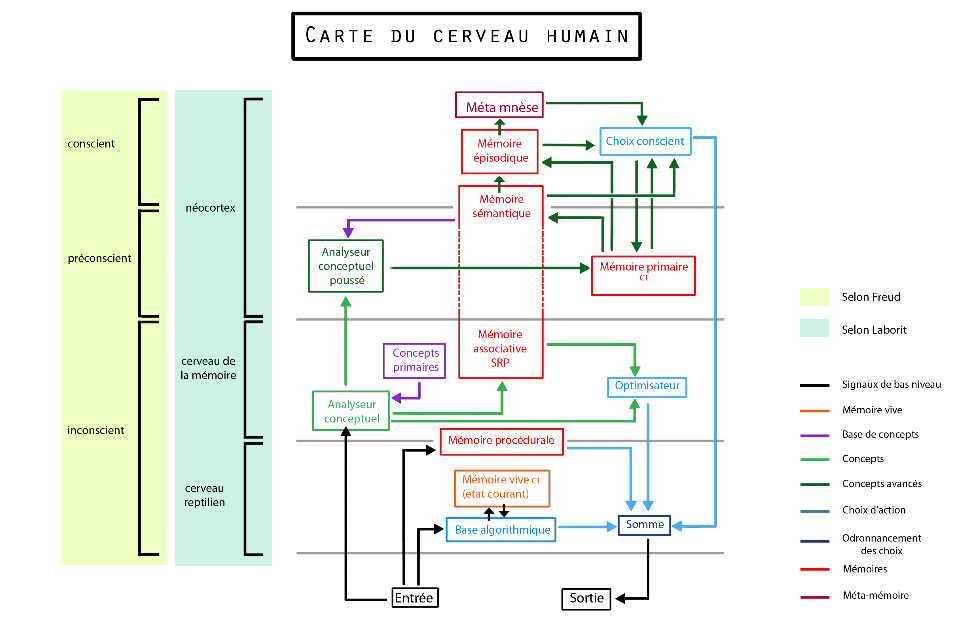
\includegraphics[width=\textwidth]{files/modele_original} 
\caption{Schéma du modèle de représentation de la conscience.} 
\label{modele_original}
\end{figure}

Cette représentation peut être vue comme un empilement de couches : l'inconscient se situant au plus bas et le conscient au plus haut.

\subsection{L'inconscient}
L'inconscient est composé de deux niveaux : le cerveau reptilien et le cerveau de la mémoire.

\subsubsection{Le cerveau reptilien}

C'est la couche la plus basse du modèle.

\paragraph{Les entrées/sorties}
Les entrées permettent au cerveau d'acquérir deux types d'informations :
\begin{itemize}
\item les percepts externes, émis par l'environnement et perçus par les cinq sens,
\item les percepts internes, comme les pulsions, etc. 
\end{itemize}

Les sorties assurent la transmission des informations produites par le cerveau au reste du corps.

\paragraph{La base algorithmique} Il s'agit d'une base simple assurant une réaction rapide à des entrées simples, en produisant des sorties simples. C'est cette partie qui stocke les réflexes innés présents chez les êtres vivants. 

\paragraph{La mémoire procédurale} Elle permet de construire des automatismes en fonction du vécu. Par exemple, selon un schéma essai échec, un bébé apprendra à marcher en utilisant sa mémoire procédurale.

\subsubsection{Le cerveau de la mémoire} Cette couche est plus
complexe que la dernière. Elle est composée d'un analyseur conceptuel, d'une mémoire
associative et d'un optimisateur.

\paragraph {L'analyseur conceptuel} Il analyse des entrées en dur à une base de
données de concepts primaires (comme la faim, la soif, le plaisir, la fatigue, la joie, une odeur
nauséabonde, un bruit violent, etc.).
\paragraph {La mémoire associative} Elle assure l'association de concepts primaires
entre eux. Elle permet par exemple à un animal vivant dans un milieu contenant des prédateurs
bruyants d’associer le concept de danger au bruit émit par le prédateur.
\paragraph {L’optimisateur} Il a pour vocation d’optimiser un concept qui peut
se traduire par le bien-être. Prenons l’exemple précédent : si l'animal sait que l’approche d’un prédateur réduit le bien-être, et que le fait de courir peut éloigner le
prédateur et donc faire remonter le bien-être, alors l'optimisateur permettra à l'animal d'inférer l’action de fuir.

\subsection{Le Néocortex : la préconscience et la conscience}
Les couches faisant partie du néocortex représentent la préconscience et la
conscience. C'est en montant dans ces éléments que l'on s'approche de la cognition humaine.

\subsubsection{Le préconscient} Cette couche est constitué d'un analyseur
conceptuel sémantique et des mémoires primaire et sémantique.

\paragraph{L'analyseur conceptuel sémantique} Il manipule des concepts d'un niveau
supérieur à ceux manipulés par l’analyseur conceptuel du cerveau de la mémoire. Il permet la
traduction de concepts primaires en concepts complexes, qui seront stockés en mémoire
sémantique.

\paragraph{La mémoire sémantique} Elle contient une base de concepts avancés, construite sous forme de treillis, permettant l'association de concepts.

\paragraph{La mémoire primaire} Cette mémoire contient un nombre de concepts
sémantiques limité. Elle joue le rôle d'une mémoire à court terme qui stocke tout ce dont la conscience est en train de manipuler. La mémoire primaire peut recevoir des informations de l’analyseur conceptuel poussé, qui lui envoie les concepts se trouvant dans l’environnement, ou directement par la réflexion consciente, qui choisit d’y stocker un concept sur lequel une réflexion est nécessaire.

\paragraph{La gestion de la mémoire sémantique} Les concepts en mémoire primaire sont instantanément copiés en mémoire sémantique. Toutes les informations qui passent en
mémoire primaire y sont transmit. Cependant, les informations accumulées peuvent être oubliées.
L'oublie d'un concept dépend de l'activité de ce dernier en mémoire primaire.

\subsubsection{Le conscient}
Cette partie regroupe les modules les plus avancés du modèle : la mémoire épisodique, la métamnèse et le choix conscient.

\paragraph{La mémoire épisodique} Il s'agit d'une mémoire des situations, qui permet la remémoration évènements et des émotions vécues sous formes de concepts sémantiques. Les concepts stockés proviennent à la fois des percepts et de l’état interne de la personne au moment de l'événement. Elle gère la persistance au même titre que la mémoire sémantique.

\paragraph{La métamnèse} C'est la mémoire de la mémoire. Son rôle est de stocker la
façon dont les éléments se sont enchaînés dans la mémoire épisodique.

\paragraph{Le choix conscient} (ou réflexion consciente) Il peut être vu comme un optimisateur de haut niveau, maniant des concepts poussés, et de natures différentes. Grâce à la métamnèse, il peut utiliser des séries de situations, et même imaginer des situations passées, présentes ou futures pour prendre des décisions. Il est ainsi capable de comparer des situations imaginaires et choisir celle vers laquelle il a envie de tendre. Il a aussi la capacité à réfléchir sur des concepts abstraits, comme sur ses réflexions passées. Il est capable d'analyser son propre fonctionnement du moment où il arrive à le retranscrire sous forme de concepts.

\subsection{Synthèse}
L’objet représenté par \textbf{Somme} dans la couche du cerveau reptilien est une simplification du schéma retour. Il représente la transformation de tous les signaux en signaux de bas niveaux, et gère leur somme pour choisir lesquels inhiber et lesquels transmettre en sortie. Son fonctionnement nécessite d'arriver à combiner les signaux entre eux. Par exemple, si une personne choisit de fumer dans le choix conscient, il doit récupérer la façon d'allumer un briquet dans la mémoire procédurale.


\clearemptydoublepage
\chapter{Où ? --FIXME}
\subsection{Une activité cognitive complète}
\subsubsection{modélisation de l'environment}
\subsubsection{planification}
\subsubsection{apprentissage}

\subsection{Domaine très étudié en IA}
\subsubsection{Algorithme Minimax}
\subsubsection{Théorème de Von Neumann}
\subsubsection{Élagage Alpha-Beta}

\subsection{Évaluation/comparaison facile}

\subsection{Convergence DECOL-IMAGINA (= I2A) }
\clearemptydoublepage
\part{Analyse}

\clearemptydoublepage
\chapter{Contraintes et restrictions}
\label{chapter:les_contraintes}
\minitoc
\section{Contraintes}

\subsection{Charge de travail}
La charge de travail est directement liée à plusieurs critères : le temps,
l'effectif disponible et les compétences de chacun des membres. L'équipe COGITO que nous 
composons et qui a réalisé ce projet est composée de
quatre étudiants en Master informatique première année (DECOL\footnote{Master
DECOL : Données Connaissances et Langage Naturel.} et IMAGINA\footnote{Master
IMAGINA : Images, Games and Intelligent Agents.}). Certaines connaissances 
nécessaires à la réalisation du projet ont été enseignée durant le semestre, ce qui nous a demandé une effort d'anticipation, d'adaptation et de réactivité. Le projet s'est déroulé du mois de Février au mois d'Avril, soit environ trois mois de réalisation, période durant laquelle devaient être effectuées les tâches
suivantes :

\begin{itemize}
\item étude du sujet, 
\item formalisation, 
\item développement, 
\item évaluation,
\item et préparation du rendu (rédaction du présent rapport et préparation de la soutenance).
\end{itemize}

Nous avons donc dû effectuer un gros travail de simplification du modèle initial en restant modeste, afin de pouvoir offrir un outil aboutit et fonctionnel à la date du rendu.

\section{Restrictions}

\subsection{Aperçu général des limitations appliquées}

La figure~\ref{modele_restreint} met en évidence le sous ensemble que nous avons choisi d'étudier, celui-ci a été déterminé à partir des contraintes énumérées au chapitre~\ref{chapter:les_contraintes}. Cette sous partie correspond à ce que Laborit nomme le néocortex, à laquelle nous avons soustrait la Méta mnèse.

\begin{figure}[H] 
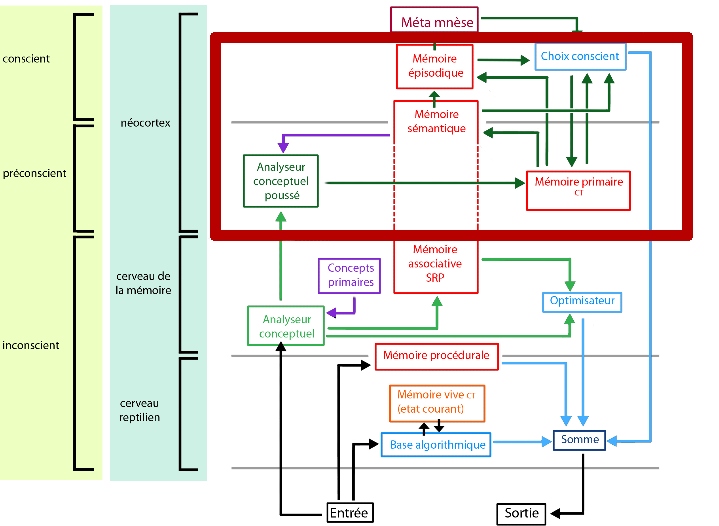
\includegraphics[width=\textwidth]{files/modele_restreint} 
\caption{Modèle restreint déterminé à partir des contraintes énumérée au chapitre~\ref{chapter:les_contraintes}} 
\label{modele_restreint}
\end{figure}

\begin{figure}[H] 
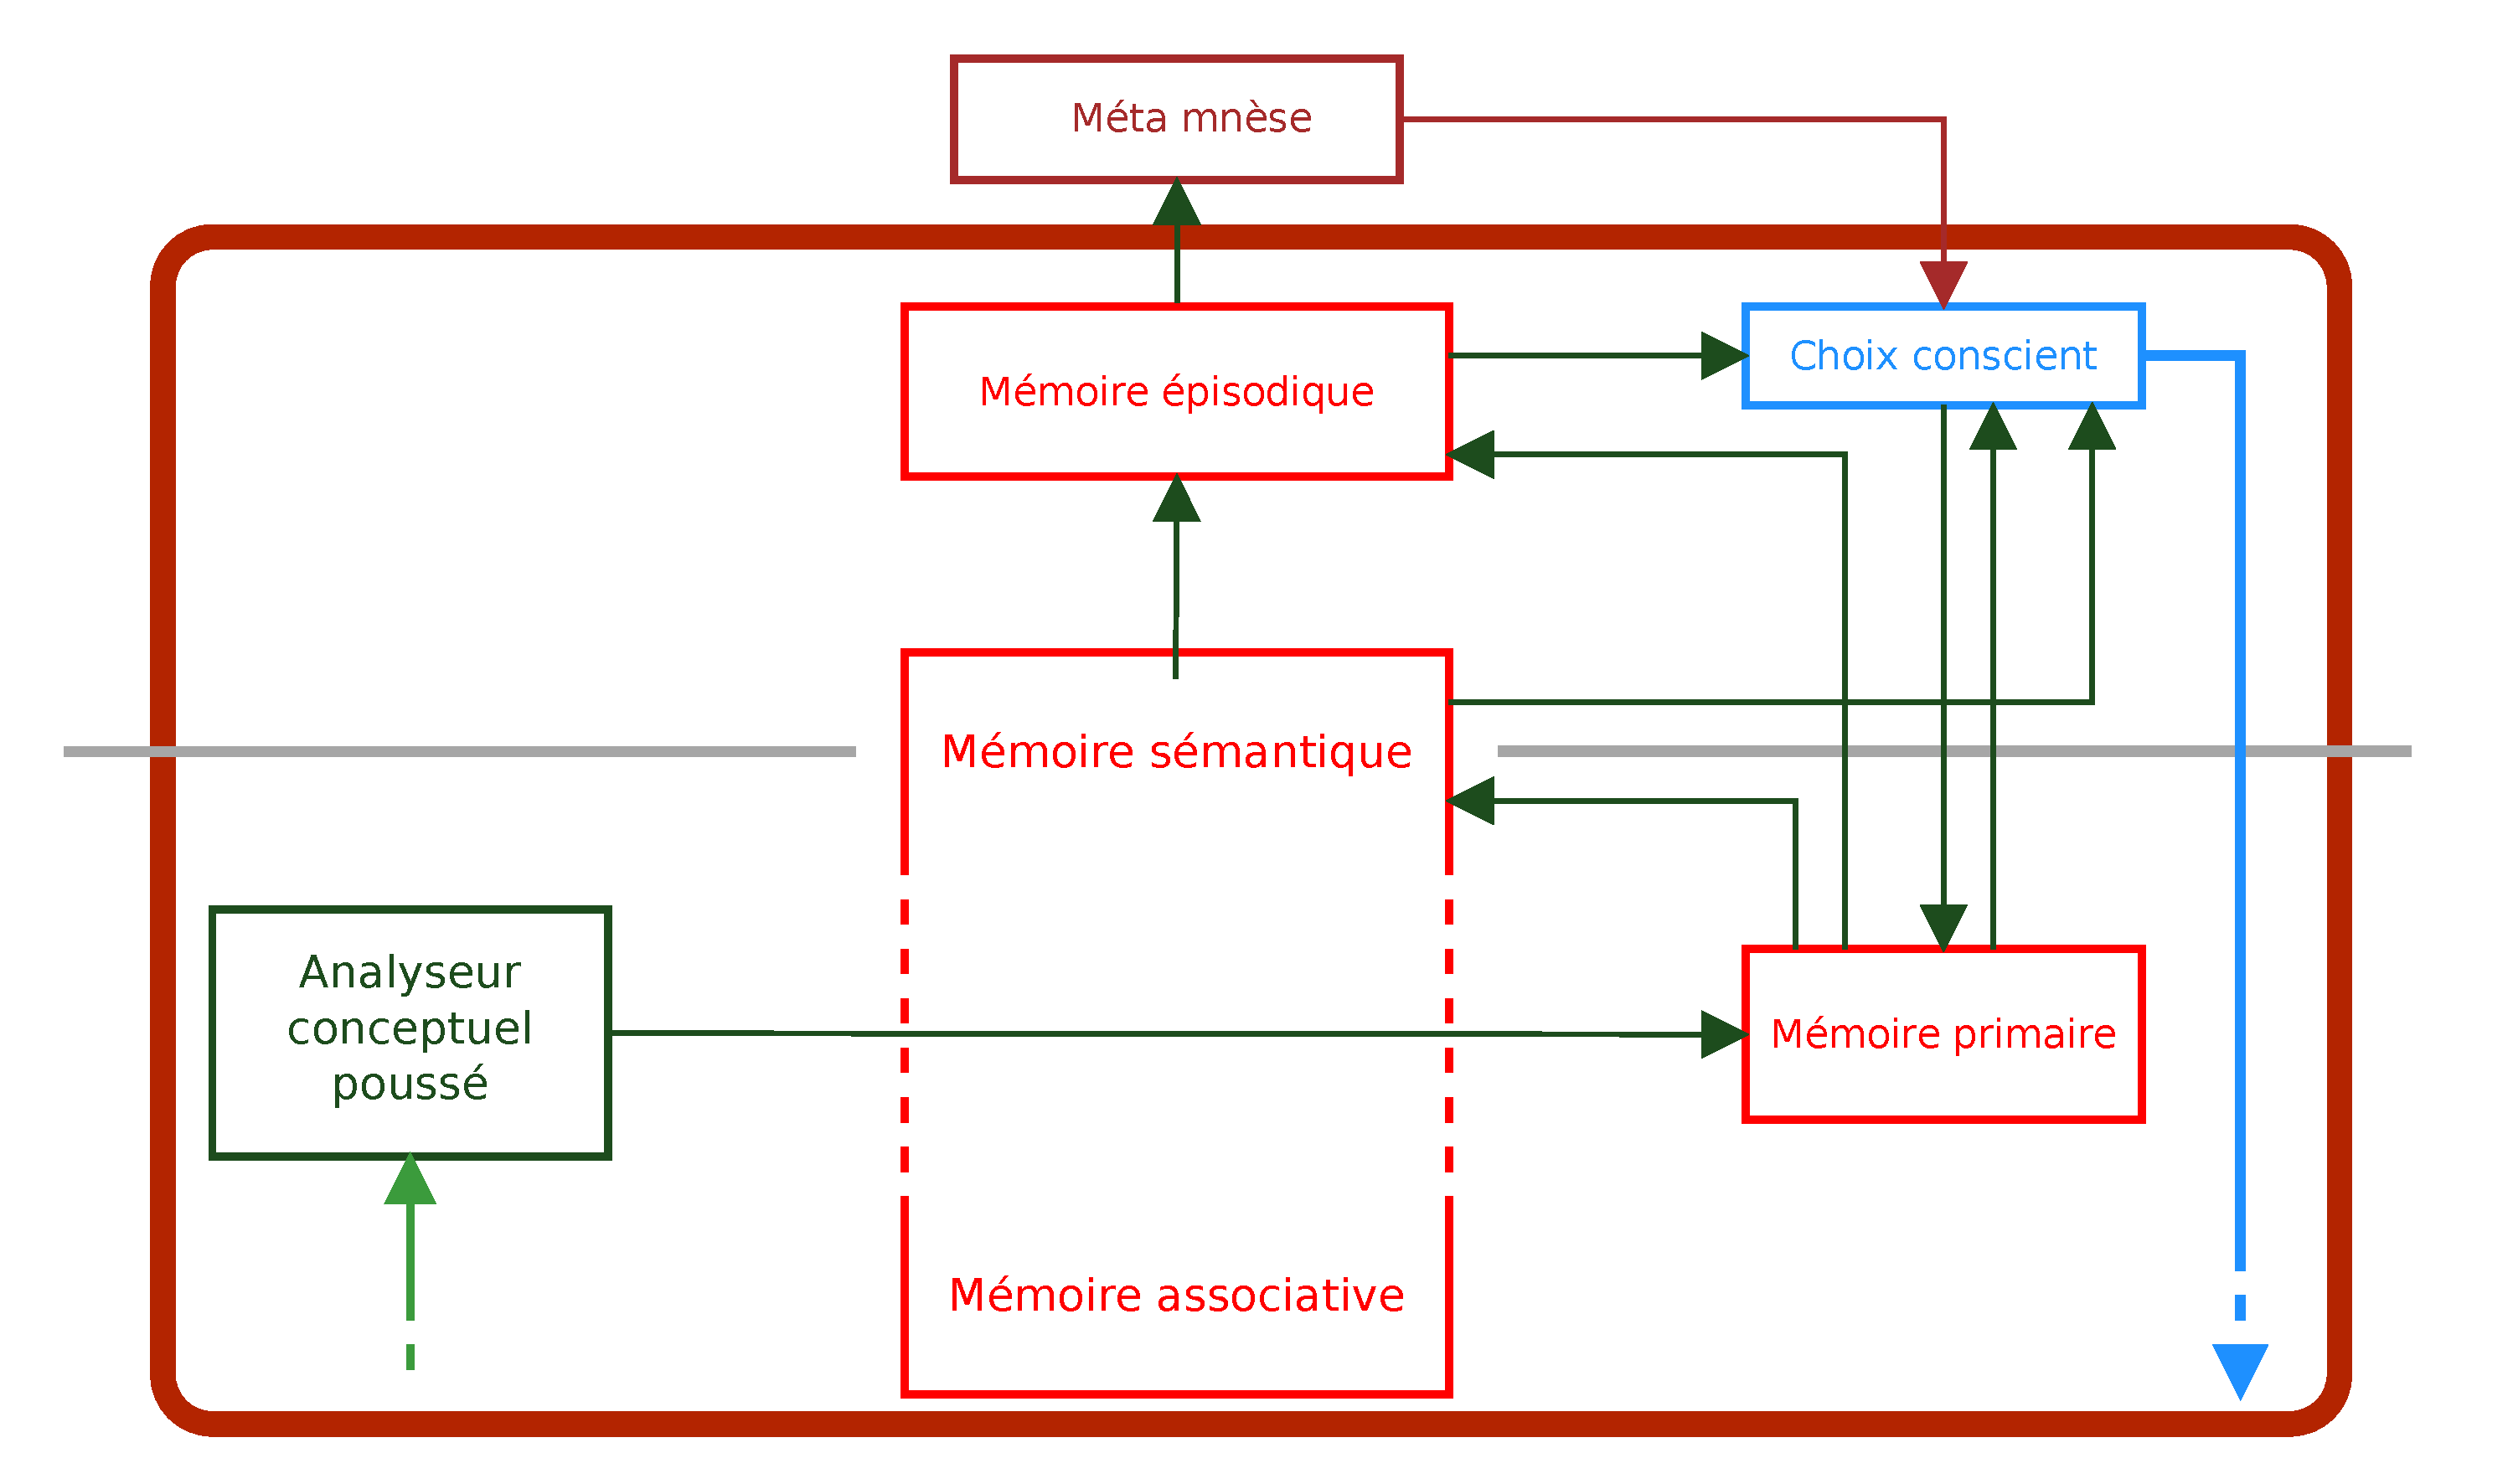
\includegraphics[width=\textwidth]{files/restricted_model_french} 
\caption{Zoom sur le  modèle restreint} 
\label{zoom_modele_restreint}
\end{figure}

\subsection{Domaine d'application : le jeu de plateau}
\label{section:domaine_application_le_jeu_de_plateau}

%----------------------------------------
% DOMAINE D'APPLICATION : POUQUOI
%----------------------------------------
\begin{frame}{Domaine d'application}{Jeu de plateau}

\begin{block}{Pourquoi le jeu de plateau ?}
\begin{itemize}
\item Convergence \texttt{DECOL} / \texttt{IMAGINA}.
\pause
\item Activité purement cognitive.
\pause
\item Activité cognitive complète.
\pause
\item Évaluation facile de la performance.
\end{itemize}
\end{block}

\end{frame}


%----------------------------------------
% LE MINIMAX
%----------------------------------------
\begin{frame}{Domaine d'application}{Théorie des jeux}

\begin{block}{Théorème du MiniMax}
\begin{itemize}
\item J. Von Neumann, 1928.
\item \textit{Stratégie optimale pour un joueur donné.}
\end{itemize}
\end{block}
\end{frame}


%----------------------------------------
% LIMITES DU MINIMAX
%----------------------------------------

\begin{frame}{Domaine d'application}{Limites du MiniMax}

\begin{block}{Type de confrontation}
\begin{itemize}
\item \underline{Minimax}: Jeux compétitifs, à deux joueurs, à somme nulle.
\item \underline{Minimax \& Nash}: Durée et nombre d'options finis.
\end{itemize}
\end{block}

\pause

\begin{block}{Temps de calcul}
\begin{itemize}
\item En moyenne \emph{$O(b^{\frac{d}{2}})$} :
	\begin{itemize}
	\item d : longeur partie.
	\item b : options par tour.
	\end{itemize}
\item En pratique : besoin d'heuristiques $\Rightarrow$ perte d'optimalité.
\end{itemize}
\end{block}

\end{frame}



\clearemptydoublepage
\chapter{Conception}
\minitoc
\begin{figure}[H] 
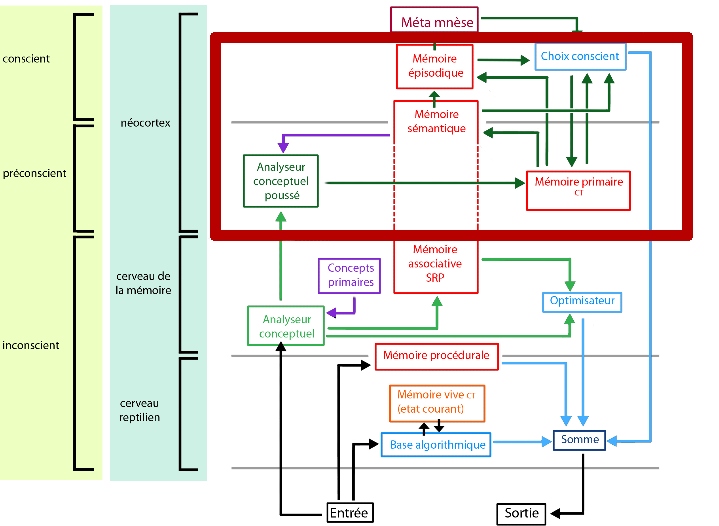
\includegraphics[width=\textwidth]{files/modele_restreint} 
\caption{Modèle restreint} 
\end{figure}

\begin{figure}[H] 
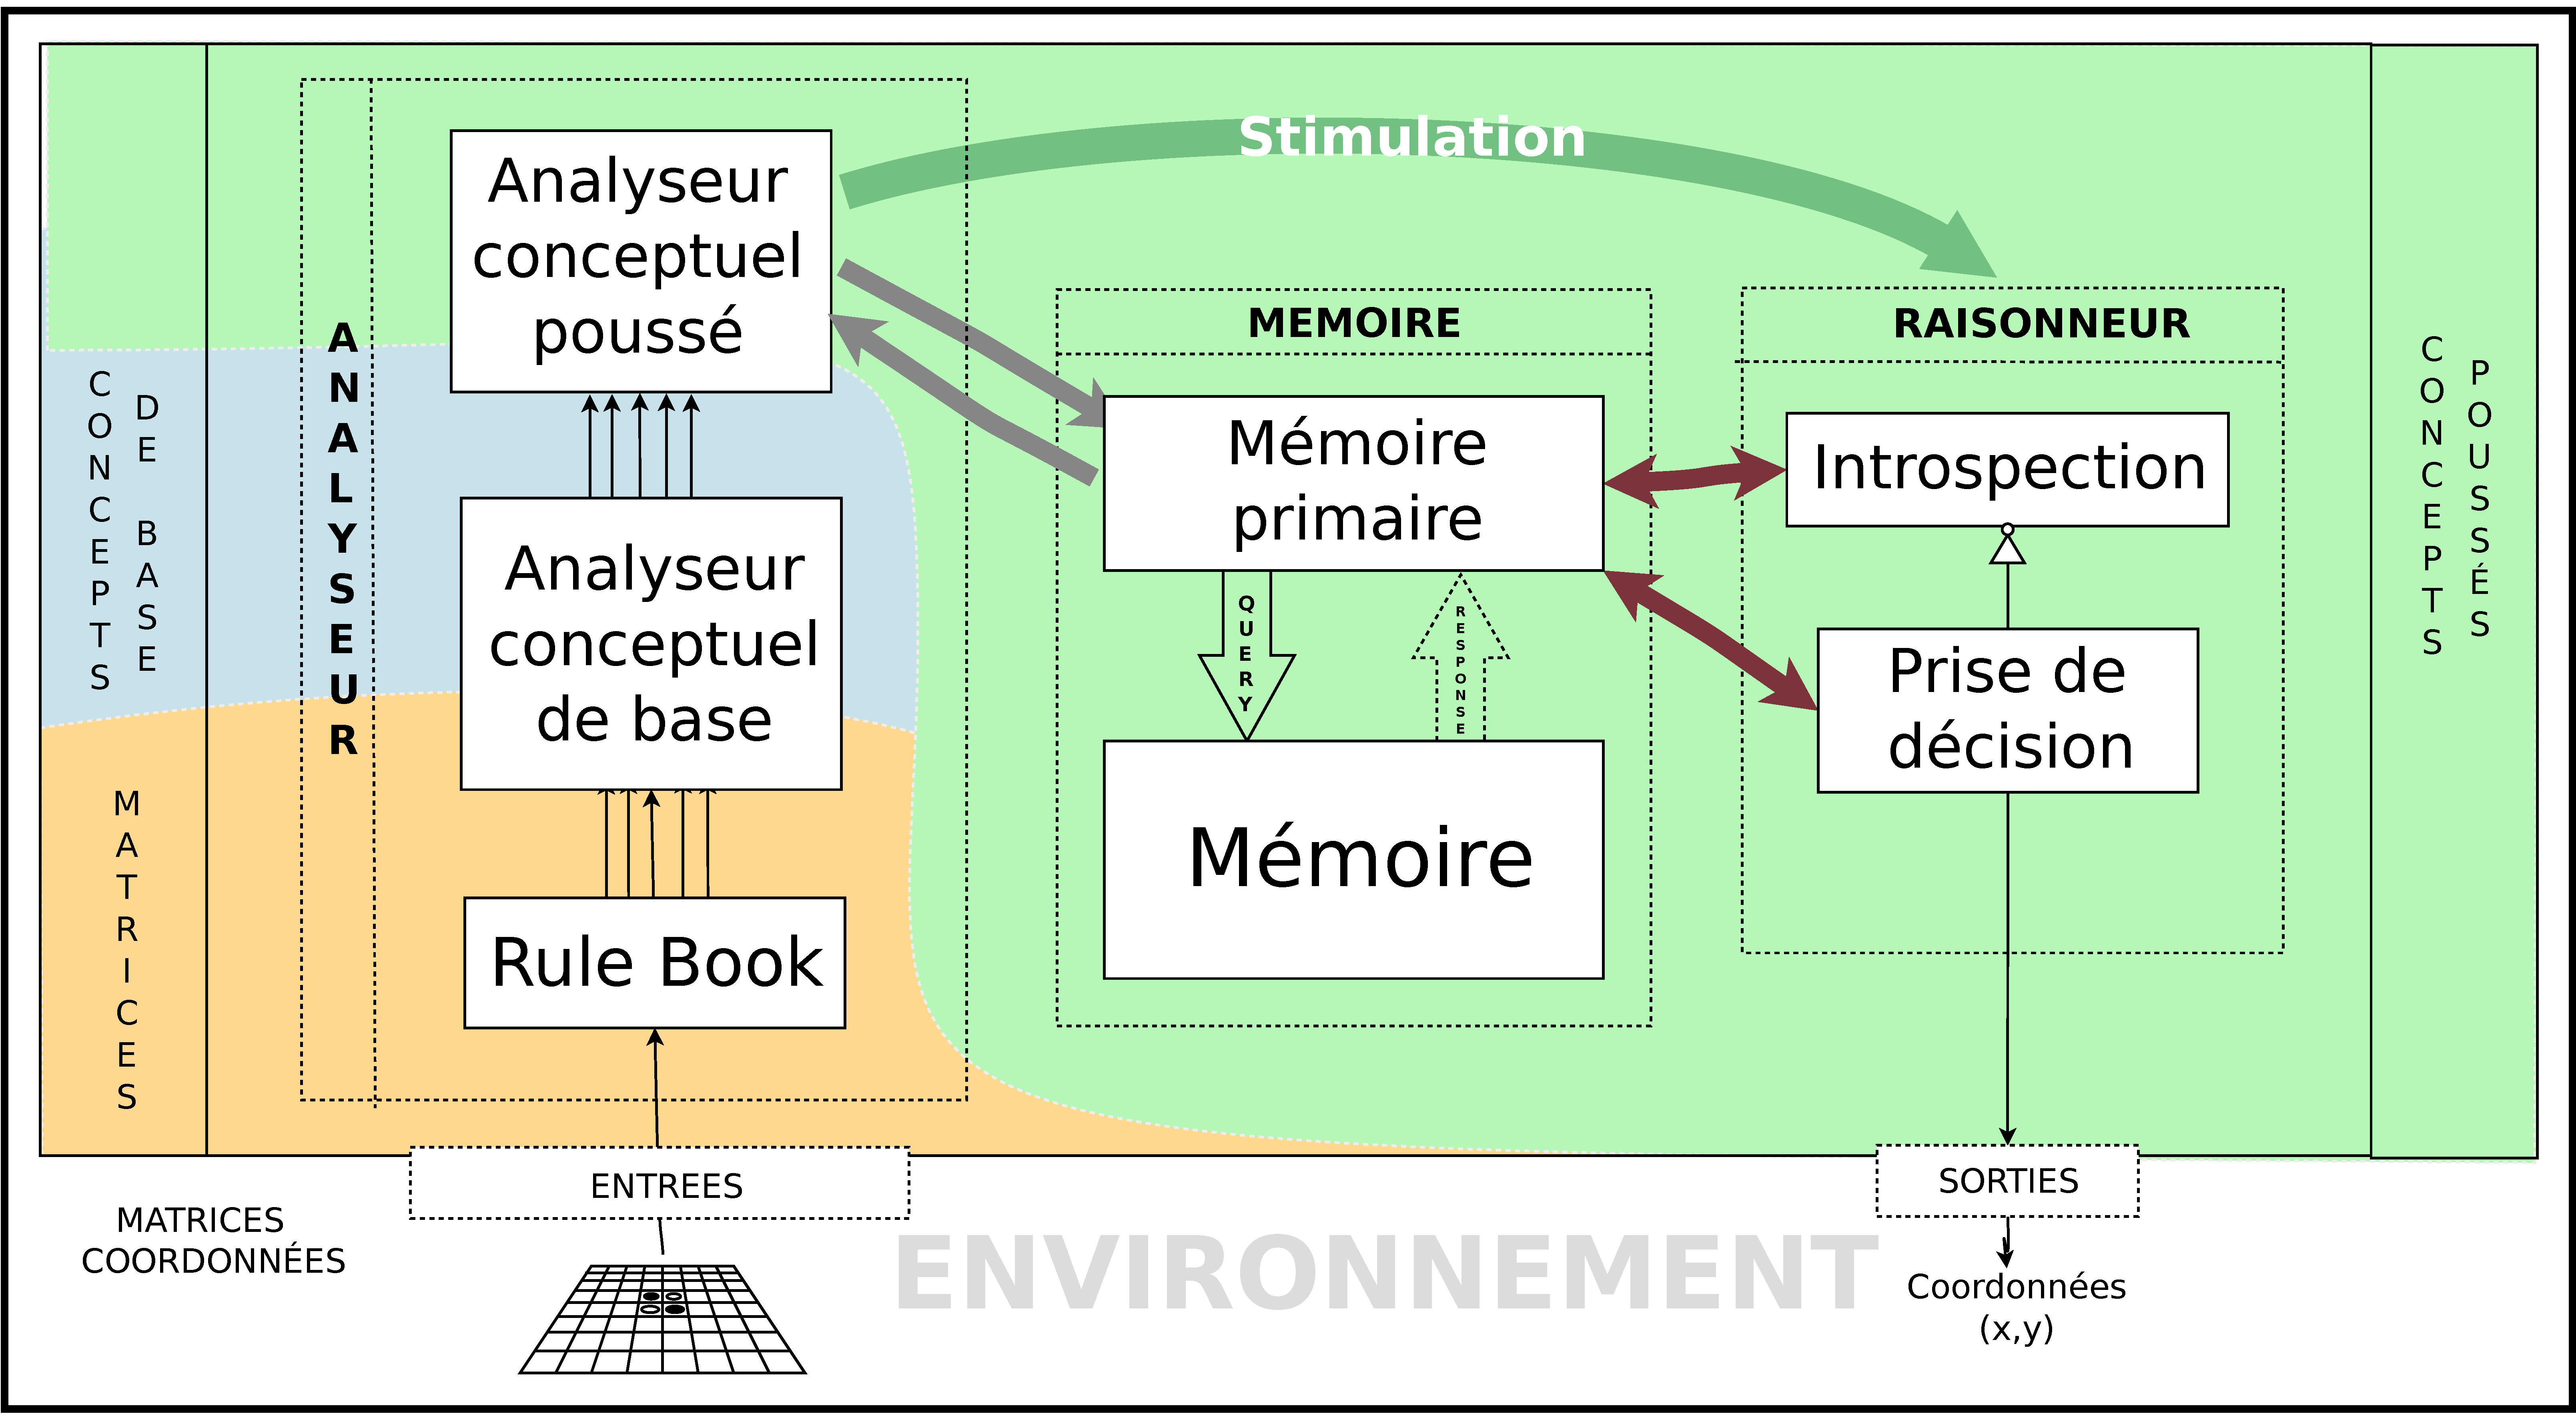
\includegraphics[width=\textwidth]{files/simplified_general_diagram} 
\caption{Schéma général} 
\end{figure}
Donec quis aliquam dolor. Mauris vitae diam sit amet urna pharetra blandit et non risus. Suspendisse velit lacus, suscipit eget feugiat a, vulputate sed sem. Ut placerat lectus sed leo vulputate at malesuada nisl cursus. Donec feugiat tempus quam, in commodo mi hendrerit sed. Ut ut mauris nisi, non ultricies lectus. Quisque lobortis ante eu dolor aliquet ut sagittis enim ultrices. Integer luctus facilisis ultricies. Nam non vestibulum turpis. Vestibulum dictum lacus quam, aliquet vulputate arcu. Donec quam nulla, condimentum vitae gravida sit amet, interdum at elit. Donec tempor eros at arcu rutrum ut tristique justo tincidunt. Nullam suscipit mauris et ligula pellentesque viverra vitae at nisi. 

\subsection{Environnement}

Ut tincidunt blandit venenatis. Praesent vel nibh vel sem viverra eleifend a rhoncus dolor. Praesent vestibulum orci mattis tellus sagittis sit amet sollicitudin elit gravida. Nam dapibus luctus tortor, ut sodales enim ultrices vel. Nulla urna urna, elementum vehicula porta ut, varius ut turpis. Vestibulum iaculis dolor sed est tempus nec imperdiet massa mollis. Ut in dignissim felis. Cras aliquet, turpis vel fermentum sollicitudin, elit nulla lobortis neque, ut tristique justo metus quis urna. Integer tincidunt, dolor ac sodales venenatis, metus dui bibendum mi, nec vehicula est neque volutpat libero. Nunc viverra rhoncus neque nec ultricies. Praesent consectetur metus et mi placerat ac fringilla sem congue. Nullam eu nisl in arcu condimentum fringilla. 

Etiam consequat, ante eget pellentesque placerat, lacus nisl facilisis lectus, nec luctus risus justo quis orci. Sed porttitor, neque quis ullamcorper venenatis, est augue convallis nisi, eu accumsan tortor magna nec urna. Aliquam erat volutpat. Nullam eget nulla nisl. Phasellus porta turpis id mauris eleifend rutrum. Suspendisse varius rhoncus magna, ut commodo ante lacinia at. Nullam viverra malesuada sapien eu luctus. 

\subsection{Module d'analyse}

Le module d'analyse est chargé de la représentation de l'environnement et de la reconnaissance de formes extraites par le module de raisonnement. Il est donc subdivisé en deux parties : \og l'analyseur conceptuel de base \fg{} et \og l'analyseur conceptuel poussé \fg{}.
\subsection{L'analyseur conceptuel de base}\label{def:analyseur de base}
Cet analyseur prend en entrée les données de l'environnement et les convertit en concepts selon un vocabulaire qui est partagé par la mémoire et le module de raisonnement. Ainsi, chaque plateau du jeu est traduit selon sa configuration en un concept qui est stocké dans la mémoire. L'analyseur conceptuel de base agit donc comme un simple traducteur.
\subsection{L'analyseur conceptuel poussé}\label{def:analyseur pousse}
Cet analyseur est chargé de la reconnaissance de formes extraites par le module de raisonnement : il génère des concepts avancés à partir de concepts simples. Il permet ainsi d'associer à chaque plateau l'ensemble de formes pertinantes qui y sont présentes. Pour ce faire, il agit comme un moteur d'inférence qui reconnait des formes par le mécanisme de recherche d'homomorphismes.


\subsection{Module de raisonnement}


Le module de raisonnement est subdivisé en deux sous modules : le \og moteur de choix \fg{} chargé de la prise de décision et le \og moteur d'introspection \fg{} chargé d'extraire de nouvelles formes remarquables.
Le moteur de choix est chargé de la partie  prise de décision du module  de raisonnement pour ce faire celui-ci sera \og stimulé \fg{} par le module d'analyse lorsque un ensemble de plateau est disponible en mémoire. Le moteur de choix doit être capable de choisir, de façon rationnel, un plateau parmi l'ensemble proposé. Pour cela, notre IA se base sur la valuation des formes remarquables (représentées sous la forme d'une formule de logique du première ordre) associées à  nos  états de plateaux possibles. En fin de partie, elle met en œuvre un mécanisme permettant la mise à jour de la valuation des différentes \og configurations \fg{} rencontrées au cours de celle-ci en fonction du résultat final de la partie.
Le moteur d'introspection est chargé de la  partie réorganisation et évaluation des \og concepts \fg{} rencontrés. Il  examine à posteriori les raisons d'une victoire où d'une défaite grâce à  la mémoire épisodique pour optimiser ses chances de victoire futur. {+ découverte nouveaux RPBS}

Le module de raisonnement est subdivisé en deux sous modules. Le premier appelé \og moteur de choix \fg{} doit être capable de choisir, de façon rationnel, un environnement parmi un ensemble proposé. Le second appelé \og raisonneur \fg{} doit être capable de trouver de nouvelles formes remarquables à partir d'une analyse de ses diverses expériences passées.

\subsubsection{Introspection}

\paragraph{Cadre Général}

Le module d'introspection a pour objectif d'extraire, à partir des expériences passées de l'IA, de nouvelles formes remarquables potentiellement discriminante pour les choix futurs. Pour ce faire, il choisi aléatoirement, en mémoire, au moins deux environnements ayant reçu la même annotations et tente d'étendre les formes déjà connues.

\begin{figure}[H] 
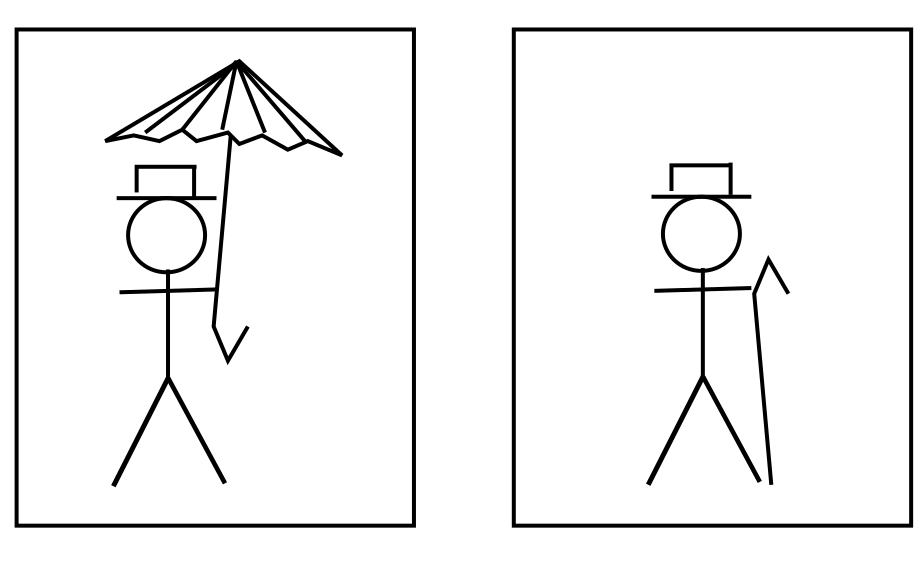
\includegraphics[width=\textwidth]{files/raisonneur/reconnaissance_de_formes_0} 
\caption{Illustration de la reconnaissance de forme} 
\label{img_reco_forme_0}
\end{figure}

Par exemple, sur la figure \ref{img_reco_forme_0}, nous considérons deux environnements présents en mémoire. Le premier représentant un homme avec un chapeau et un parapluie, le second un homme avec un chapeau et une canne. Nous souhaitons extraire de ces deux environnements la forme \og homme avec un chapeau \fg{}. Pour ce faire, ce module se base, sur les connaissances, présentent en mémoire relatives à ces environnements. En l'occurrence, nous considérerons que notre IA sait déjà reconnaître un homme et les a reconnu sur ces environnements. Notre module cherche alors à étendre, le plus possible, la forme \og homme \fg dans un des deux environnements tout en vérifiant que cette forme étendu peux toujours être injectée dans l'autre environnement, comme illustré dans la figure \ref{img_reco_forme_injection}.

\begin{figure}[H] 
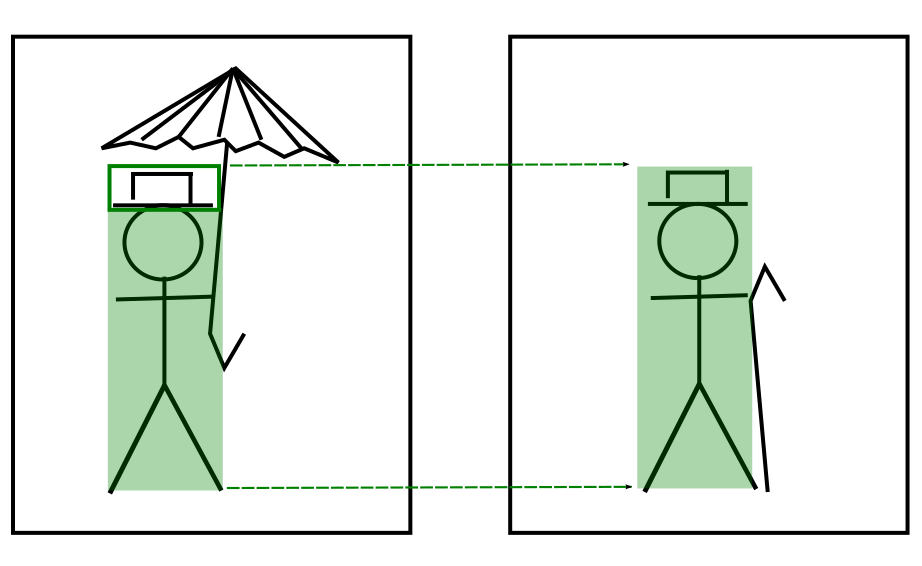
\includegraphics[width=\textwidth]{files/raisonneur/reconnaissance_de_formes_injection} 
\caption{Illustration de l'injection} 
\label{img_reco_forme_injection}
\end{figure}

\paragraph{Application aux jeux de plateau}

\begin{figure}[H] 
\begin{center}
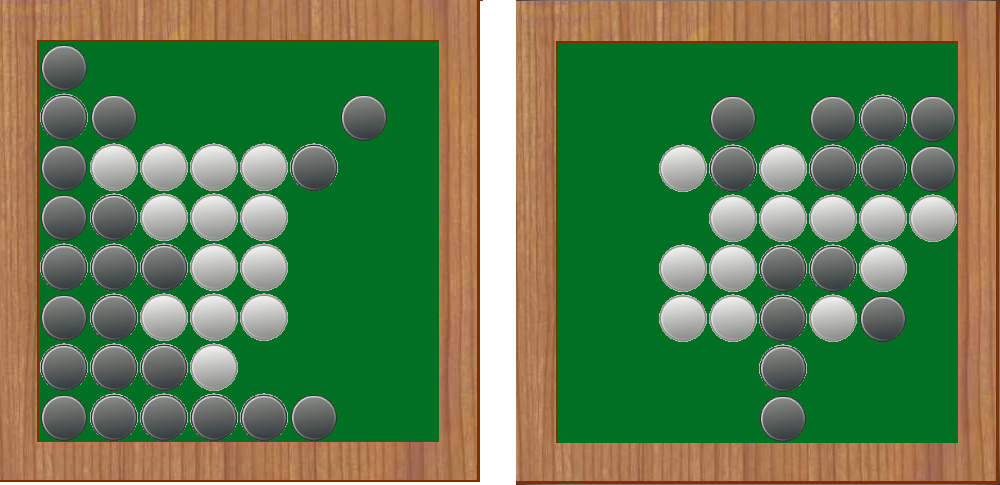
\includegraphics[width=0.7\textwidth]{files/raisonneur/cbs_reco0} 
\end{center}
\caption{Illustration de l'injection} 
\label{img_cbs_reco0}
\end{figure}

\begin{figure}[H] 
\begin{center}
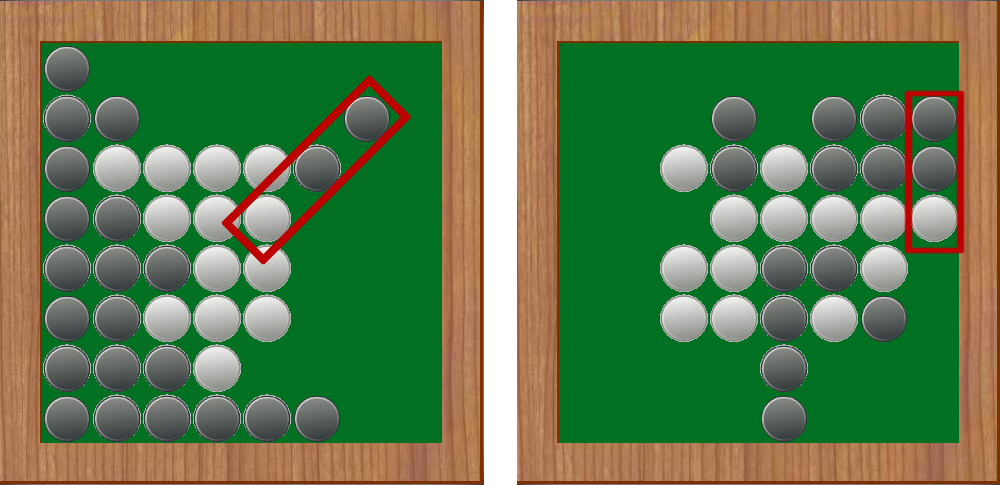
\includegraphics[width=0.7\textwidth]{files/raisonneur/cbs_reco1} 
\end{center}
\caption{Illustration de l'injection} 
\label{img_cbs_reco1}
\end{figure}

\begin{figure}[H] 
\begin{center}
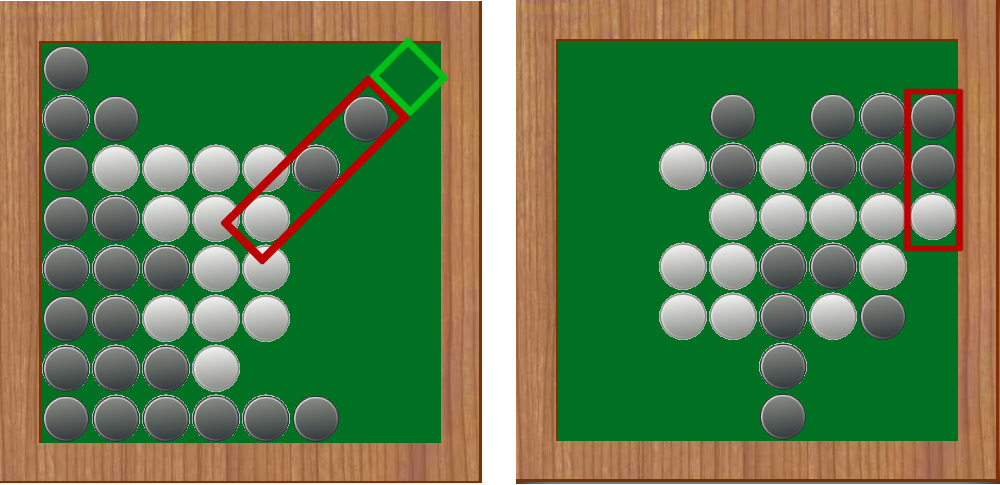
\includegraphics[width=0.7\textwidth]{files/raisonneur/cbs_reco2} 
\end{center}
\caption{Illustration de l'injection} 
\label{img_cbs_reco2}
\end{figure}

\begin{figure}[H] 
\begin{center}
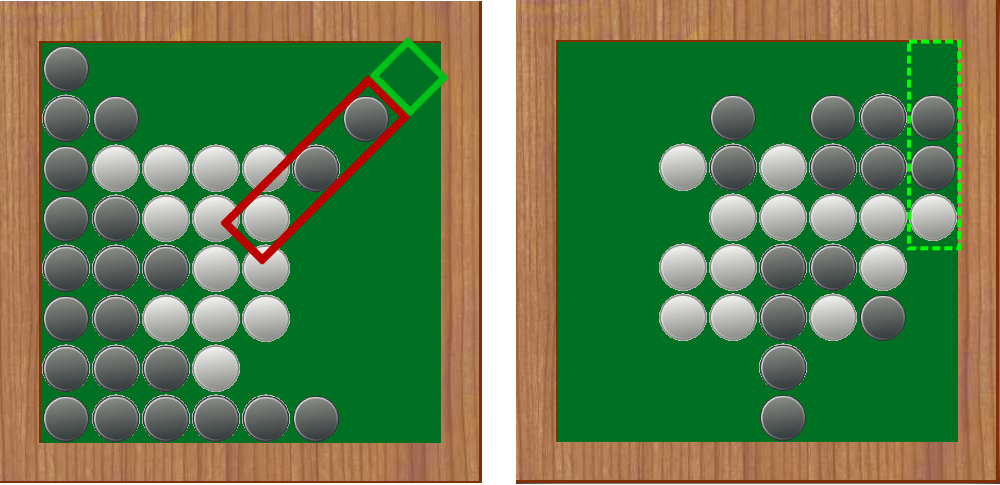
\includegraphics[width=0.7\textwidth]{files/raisonneur/cbs_reco3} 
\end{center}
\caption{Illustration de l'injection} 
\label{img_cbs_reco3}
\end{figure}

\subsubsection{Valuation des formes}

À chaque fois que le module reçoit une annotation, celui-ci effectue une mise à jour des probabilité
\[ P(Annotation|Forme) = \frac{P(Annotation|Gain) \times P(Gain)}{P(Annotation)} \]

Par exemple, imaginons que nous souhaitons entraîner notre IA à identifier des formes géométrique basique : rond, carré, croix et triangle. Admettons que notre IA est capable de reconnaître dans son environnement les formes correspondantes mais qu'elle ne sait pas les associer au concept correspondant. Nous pouvons représenter cette état par le tableau représenté en figure \ref{img_annotations}.

\begin{figure}[H] 
  \begin{center}
    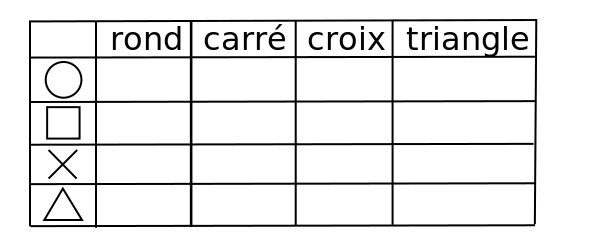
\includegraphics[width=0.5\textwidth]{files/raisonneur/annotations} 
  \end{center}
\caption{Association forme-concept} 
\label{img_annotations}
\end{figure}

\begin{figure}[H] 
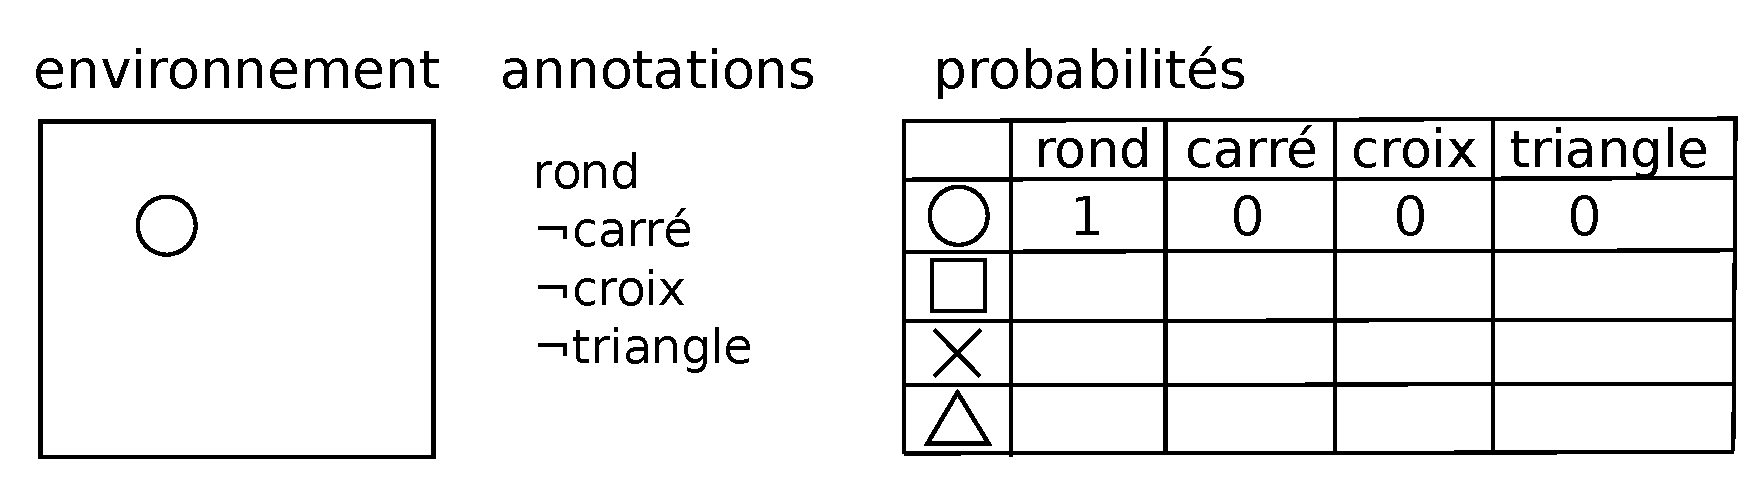
\includegraphics[width=\textwidth]{files/raisonneur/annotations_1} 
\caption{Association forme-concept 1} 
\label{img_annotations_1}
\end{figure}

\begin{figure}[H] 
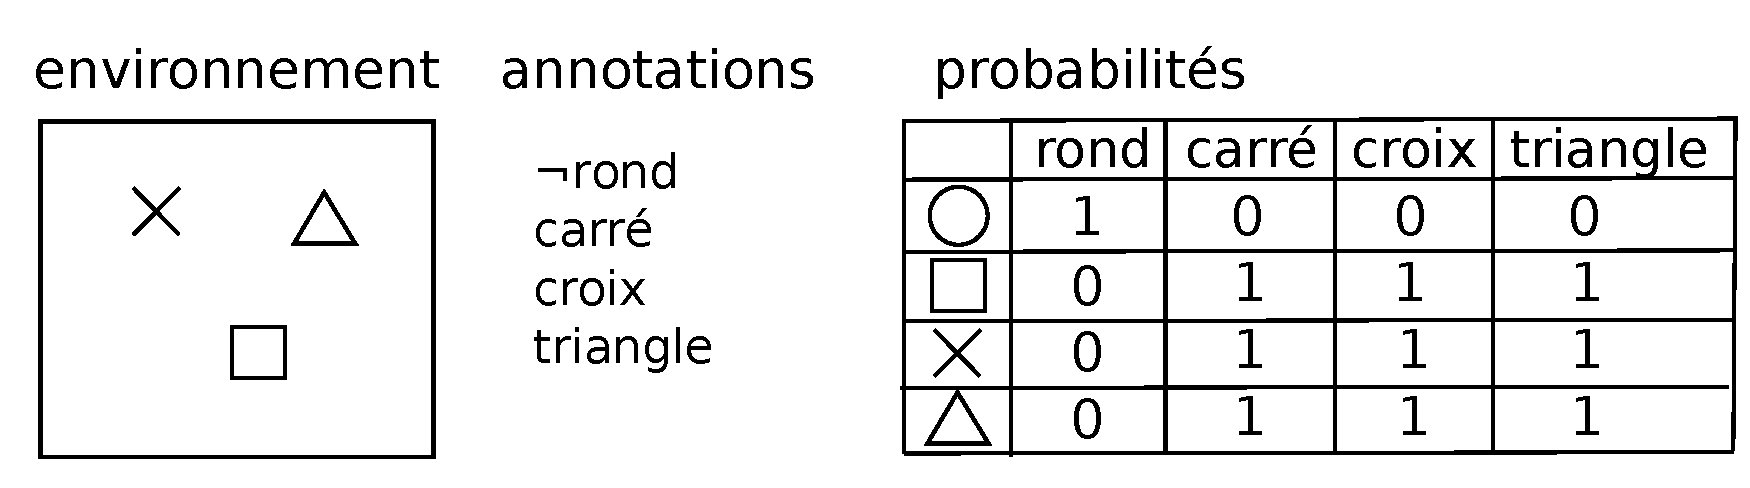
\includegraphics[width=\textwidth]{files/raisonneur/annotations_2} 
\caption{Association forme-concept 2} 
\label{img_annotations_2}
\end{figure}

\begin{figure}[H] 
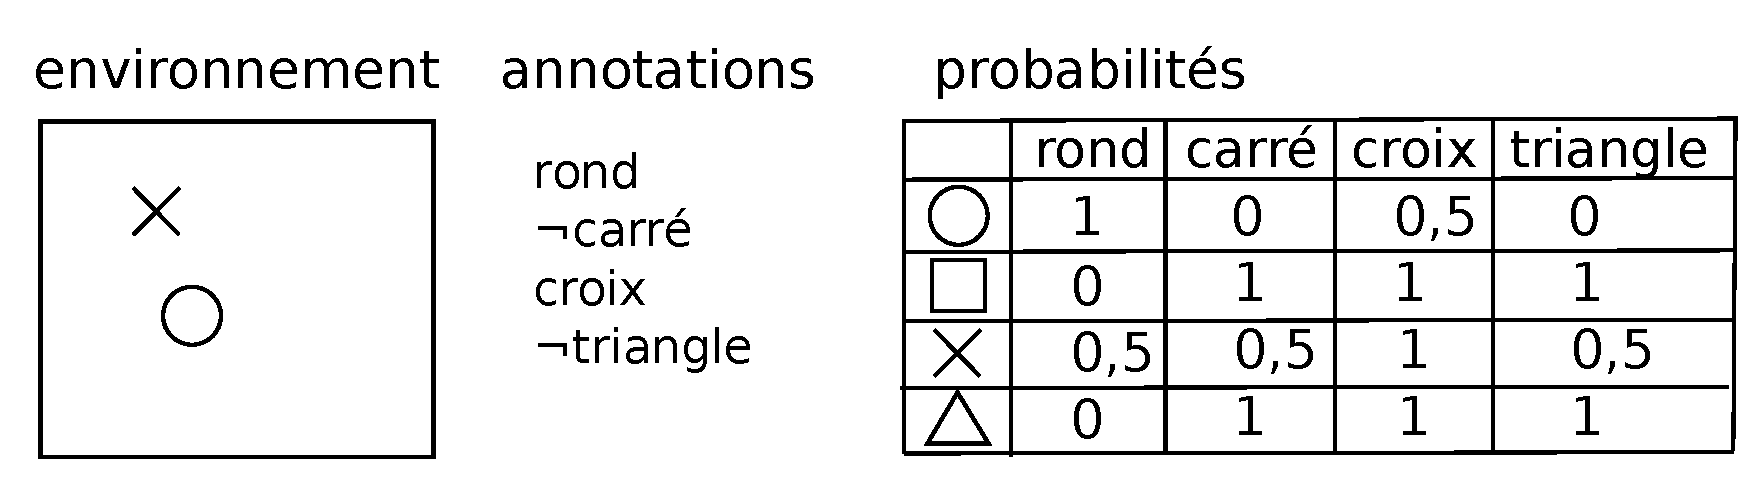
\includegraphics[width=\textwidth]{files/raisonneur/annotations_3} 
\caption{Association forme-concept 3} 
\label{img_annotations_3}
\end{figure}

\begin{figure}[H] 
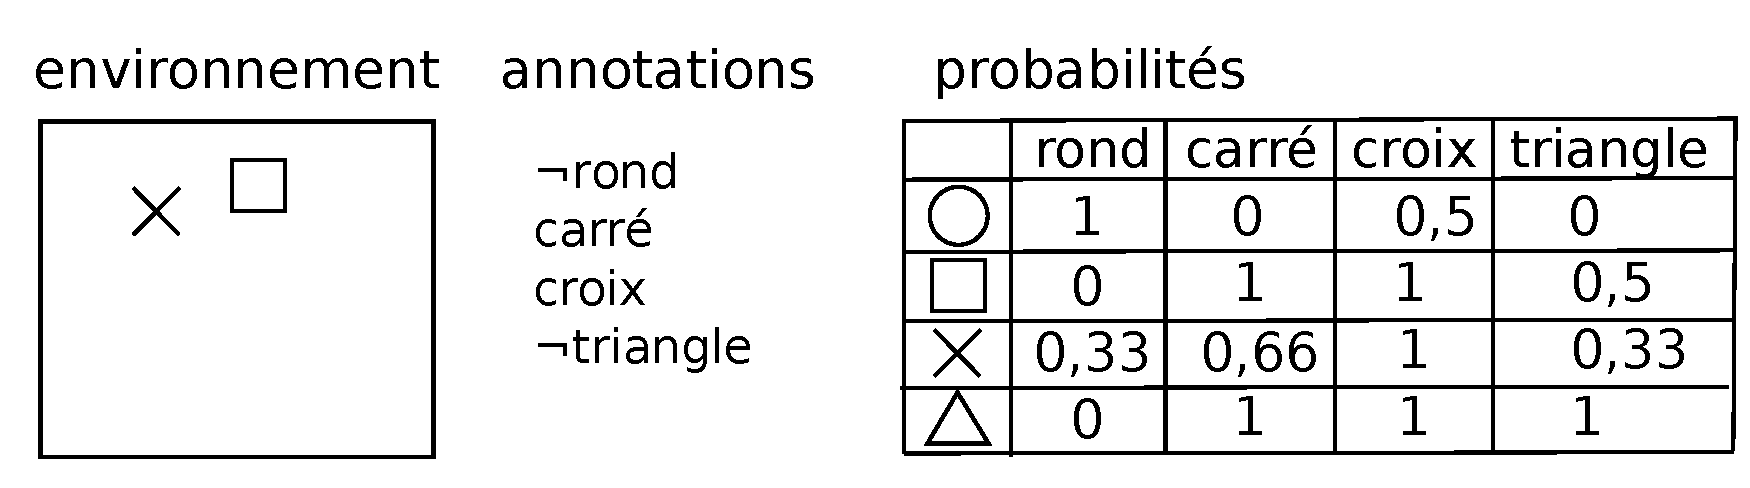
\includegraphics[width=\textwidth]{files/raisonneur/annotations_4} 
\caption{Association forme-concept 4} 
\label{img_annotations_4}
\end{figure}

\begin{figure}[H] 
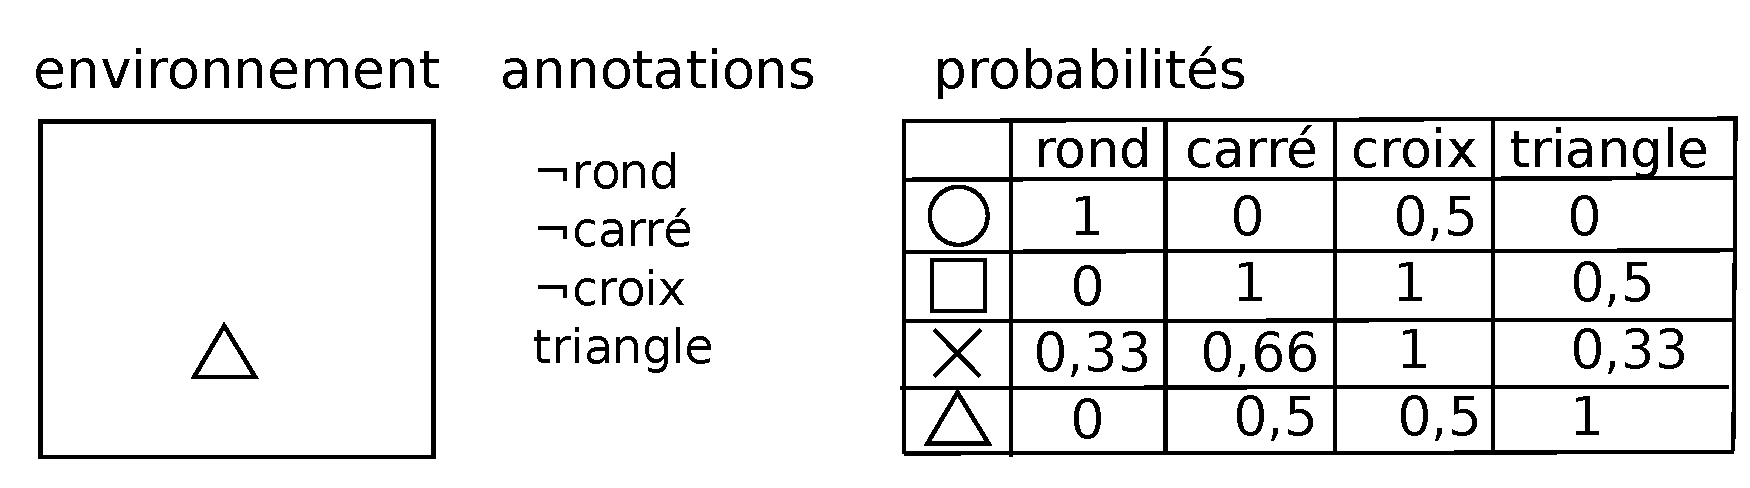
\includegraphics[width=\textwidth]{files/raisonneur/annotations_5} 
\caption{Association forme-concept 5} 
\label{img_annotations_5}
\end{figure}



\subsubsection{Moteur de choix}

\paragraph{Cadre Général}


Ce module intervient après la phase d'analyse qui lui fourni, par l'intermédiaire de la mémoire, un ensemble d'environnements possibles et pour chacun d'eux un ensemble de formes reconnues. Le \og moteur de choix \fg{} se sert alors de la probabilité d'apparition des annotations associées aux formes reconnu afin d'évaluer chaque environnement possible. Il choisi finalement l'environnement qui maximise sa fonction objectif.

\paragraph{Application aux jeux de plateau}


\begin{figure}[H] 
  \begin{center}
		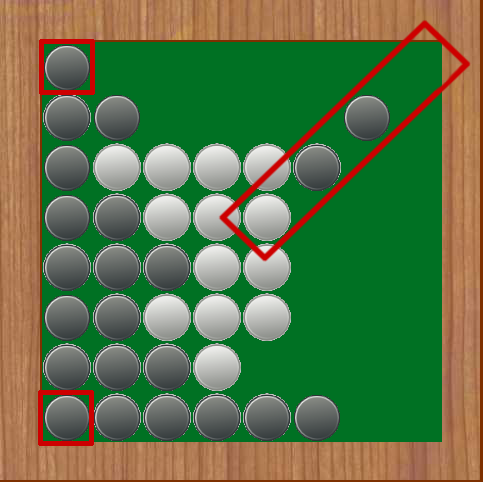
\includegraphics[width=0.3\textwidth]{files/raisonneur/moteur_de_choix} 
	\end{center}
\caption{Représentation graphique de l'environnement} 
\label{img_env}
\end{figure}


\subsubsection{Moteur d'introspection}

\subsection{Mémoires}

\subsubsection{Interface Mémoire}

Le module de mémoire a été conçu de manière générique à l'aide d'interfaces java. Pour cela elle se décompose en trois parties :

\begin{itemize}
\item l'interface principale de la mémoire, qui déclare les méthodes appelées par les autres modules (Analyse et Raisonnement), et qui est implémentée en tant que mémoire à court terme (ActiveMemory),

\item l'interface de la mémoire épisodique et l'interface de la mémoire sémantique, qui déclarent les méthodes appelées par le module Mémoire.
\end{itemize}

\begin{figure}[H]
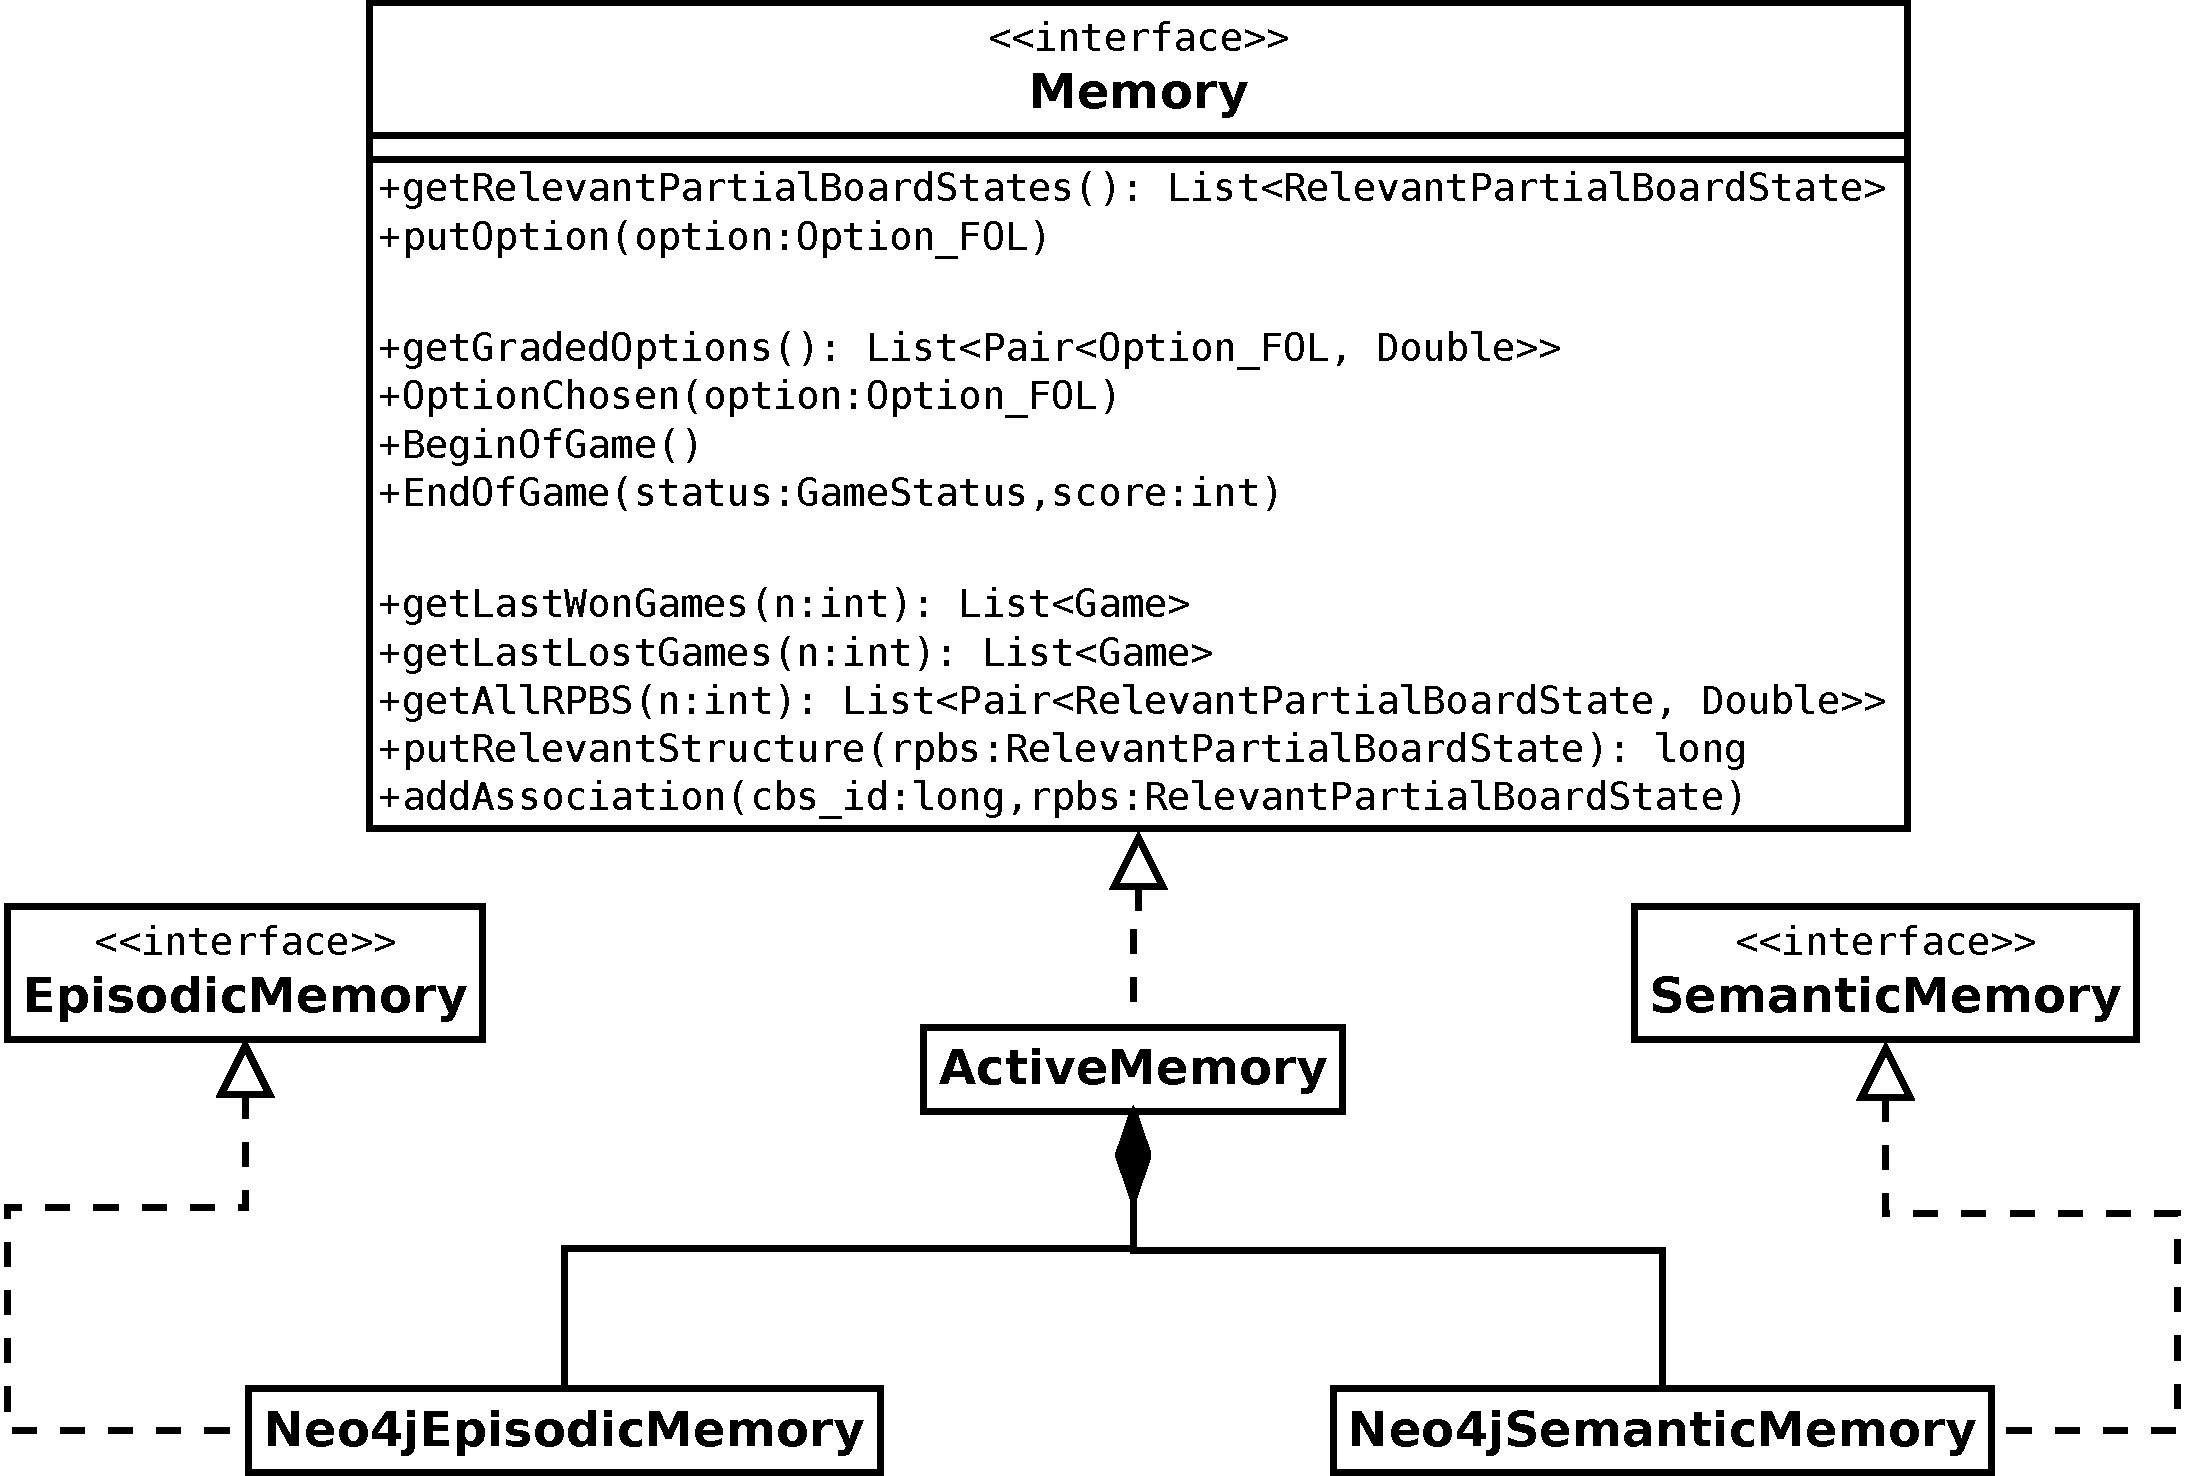
\includegraphics[width=\textwidth]{files/memoire/interface}
\caption{Interface mémoire}
\end{figure}

La mémoire doit également assurer la persistance des données, qui se fait via un module de persistance. Celui-ci est utilisé par une implémentation spécifique des interfaces décrites ci-avant.

\subsubsection{Le \gls{SGBD} Neo4j}

La persistance des données est assurée par un SGBD né de la mouvance \gls{NoSQL} : Neo4j. Il permet la gestion d'une base de données orientée graphe. Nous avons fait le choix d'utiliser un tel système pour plusieurs raisons :

\begin{itemize}
\item nous avions la volonté de découvrir une solution \gls{NoSQL}, que nous n'avons pas eu l'occasion d'étudier lors de notre formation,

\item Neo4j est disponible en plusieurs versions, notamment en version serveur, version webservice REST et version java embarquée. La mémoire n'étant pas accédée de manière concurrente ainsi que pour des soucis de légèreté, c'est la version embarquée (\emph{embedded java})qui a été utilisée,

\item ce type de \gls{SGBD} \gls{NoSQL} permet d'obtenir des temps d'accès plus rapides qu'avec des \gls{SGBD} relationnels traditionnels,

\item la vision graphe de la base de données est adaptée à la conception de notre mémoire\footnote{Notons tout de même qu'il aurait était été possible de stocker les données sous forme de tables},

\item cette solution conserve les propriétés \gls{ACID} des transactions des \gls{SGBD} relationnels traditionnels,

\item la documentation complète et la communauté active permettent de s'initier très rapidement à cette nouvelle technologie,

\item Neo4j est une solution libre distribuée sous licence \gls{GPLv3}.
\end{itemize}

Neo4j étant un \gls{SGBD} \gls{NoSQL} orienté graphe, la base de donnée est représentée sous la forme d'un graphe orienté, composé d'un nœud \og root \fg{}. Chaque nœud et chaque arc peut posséder des attributs. Cependant, il n'est possible de définir que des types d'arc, pour les nœuds on utilise donc une astuce qui consiste en la création d'un \og master\_node \fg{} comme le montre le schéma suivant : 

\begin{figure}[H]
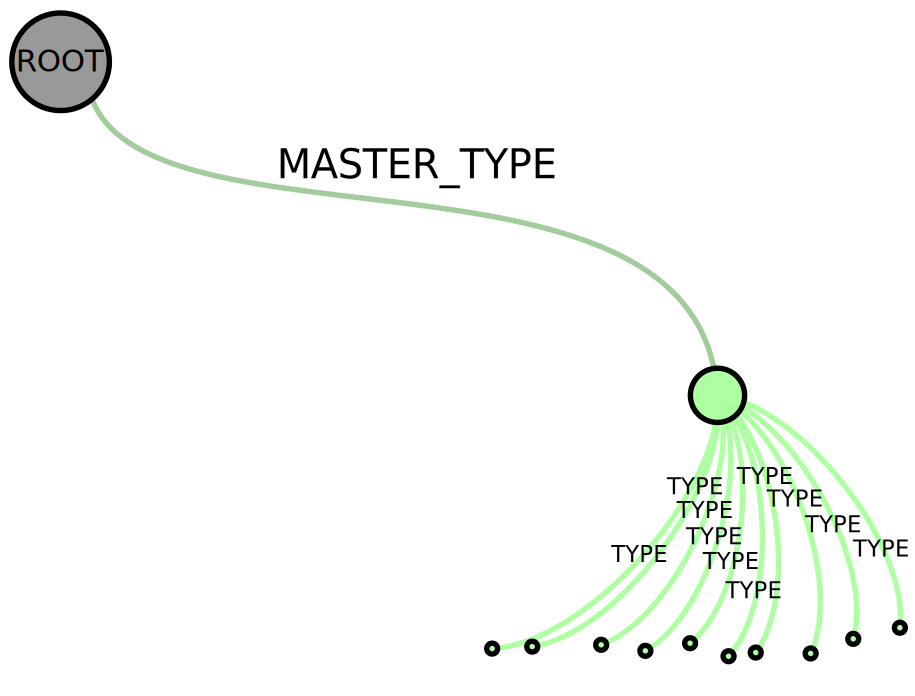
\includegraphics[width=\textwidth]{files/neo4j/example_node_type}
\caption{Exemple de typage des noeuds avec Neo4j.}
\label{example_node_type}
\end{figure}

\subsubsection{Éléments en mémoire}

Le module de persistance permet le stockage de la mémoire épisodique et sémantique, les deux étant liées par les relations entre les \emph{MOVE} et les \emph{CBS}. Nous avons donc besoin des types suivants : 

\textbf{Types de noeud :}
\begin{itemize}
	\item \texttt{GAME} : une partie en mémoire épisodique, 
	\item \texttt{MOVE} : un coup joué en mémoire épisodique,
	\item \texttt{CBS} : un \texttt{CBS} en mémoire sémantique,
	\item \texttt{RPBS} : un \texttt{RPBS} en mémoire sémantique.
\end{itemize}


\textbf{Types de liens :}
\begin{itemize}
	\item Relations maitres
		\begin{itemize}
			\item \texttt{MASTER\_ATTR},
			\item \texttt{MASTER\_OBJ},
			\item \texttt{MASTER\_GAME},
			\item \texttt{MASTER\_MOVE}.
		\end{itemize}
	\item Relations de type
		\begin{itemize}
			\item \texttt{ATTRIBUTE},
			\item \texttt{OBJECT},
			\item \texttt{MOVE},
			\item \texttt{GAME},
			\item \texttt{LAST\_GAME} (relation \texttt{GAME} spéciale, signifiant que cette partie est la dernière jouée).
		\end{itemize}
	\item Relations en mémoire épisodique
		\begin{itemize}
			\item \texttt{PREV\_GAME} : permet à partir d'une partie d'accéder à la précédente,
			\item \texttt{LAST\_MOVE} : permet à partir d'une partie d'accéder au dernier coup joué,
			\item \texttt{PREV\_MOVE} : permet à partir d'un coup d'accéder au précédent,
			\item \texttt{STATE\_BOARD} : permet de lier un coup à l'état de plateau correspondant.
		\end{itemize}
	\item Relations en mémoire sémantique
		\begin{itemize}
			\item \texttt{RELATED} : décrit la présence d'un \texttt{RPBS} dans un \texttt{CBS}.
		\end{itemize}
	\end{itemize}
	
\subsubsection{Mémoire sémantique}
Comme vu dans la partie~\ref{conception_memoire_semantique} (page \pageref{conception_memoire_semantique}, la mémoire sémantique stocke une matrice de booléens ayant comme attributs (colonnes) des \texttt{RPBS}, et comme objets (lignes) des \texttt{CBS}.

On peut voir sur la figure~\ref{lattice_graph} les deux \og master\_node \fg{} permettant de déclarer des nœuds d'attributs et d'objets. Ces noeuds sont en liés via des relations de type \emph{RELATED}.

\begin{figure}[H]
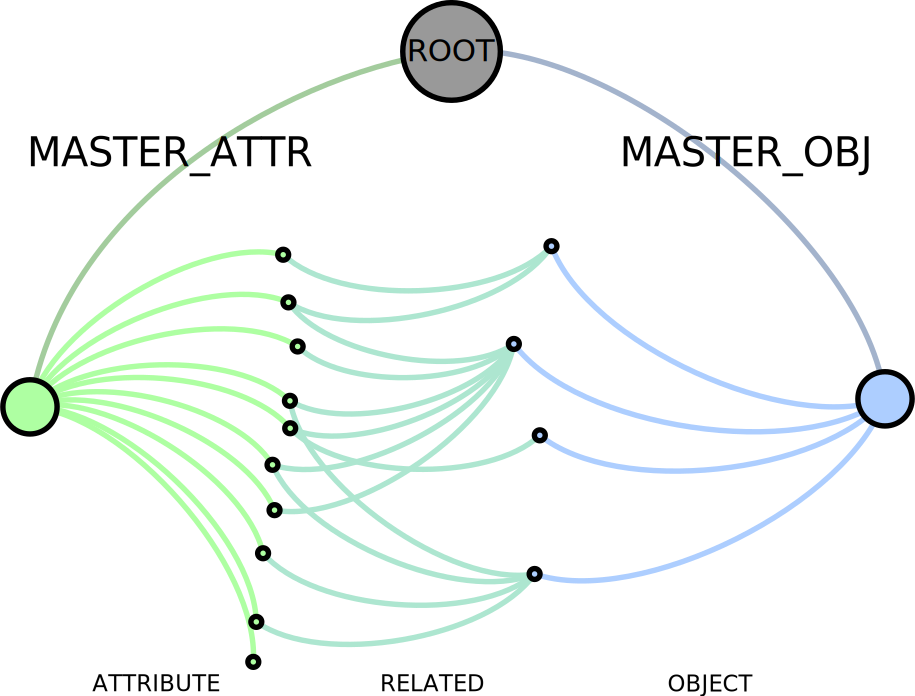
\includegraphics[width=\textwidth]{files/neo4j/lattice_graph}
\caption{Représentation de la mémoire sémantique dans Neo4j.}
\label{lattice_graph}
\end{figure}

\subsubsection{Mémoire épisodique}

La représentation sous forme de graphe se prête parfaitement à la mémorisation des parties et des coups sous la forme d'une double liste chaînée. La figure~\ref{episodic_graph} représente la mémoire épisodique telle qu'elle est stockée dans Neo4j.

On visualise parfaitement les trois \og master\_node \fg{} permettant de typer les \texttt{GAME}, \texttt{MOVE} et \texttt{ATTRIBUTES}. Le parcours des parties se fait via la relation \texttt{PREV\_GAME} et celui des coups via la relation \texttt{PREV\_MOVE}.

On remarque également que les relations \texttt{BOARD\_STATE} permettent de faire la liaison entre la mémoire sémantique et la mémoire épisodique.

\begin{figure}[H]
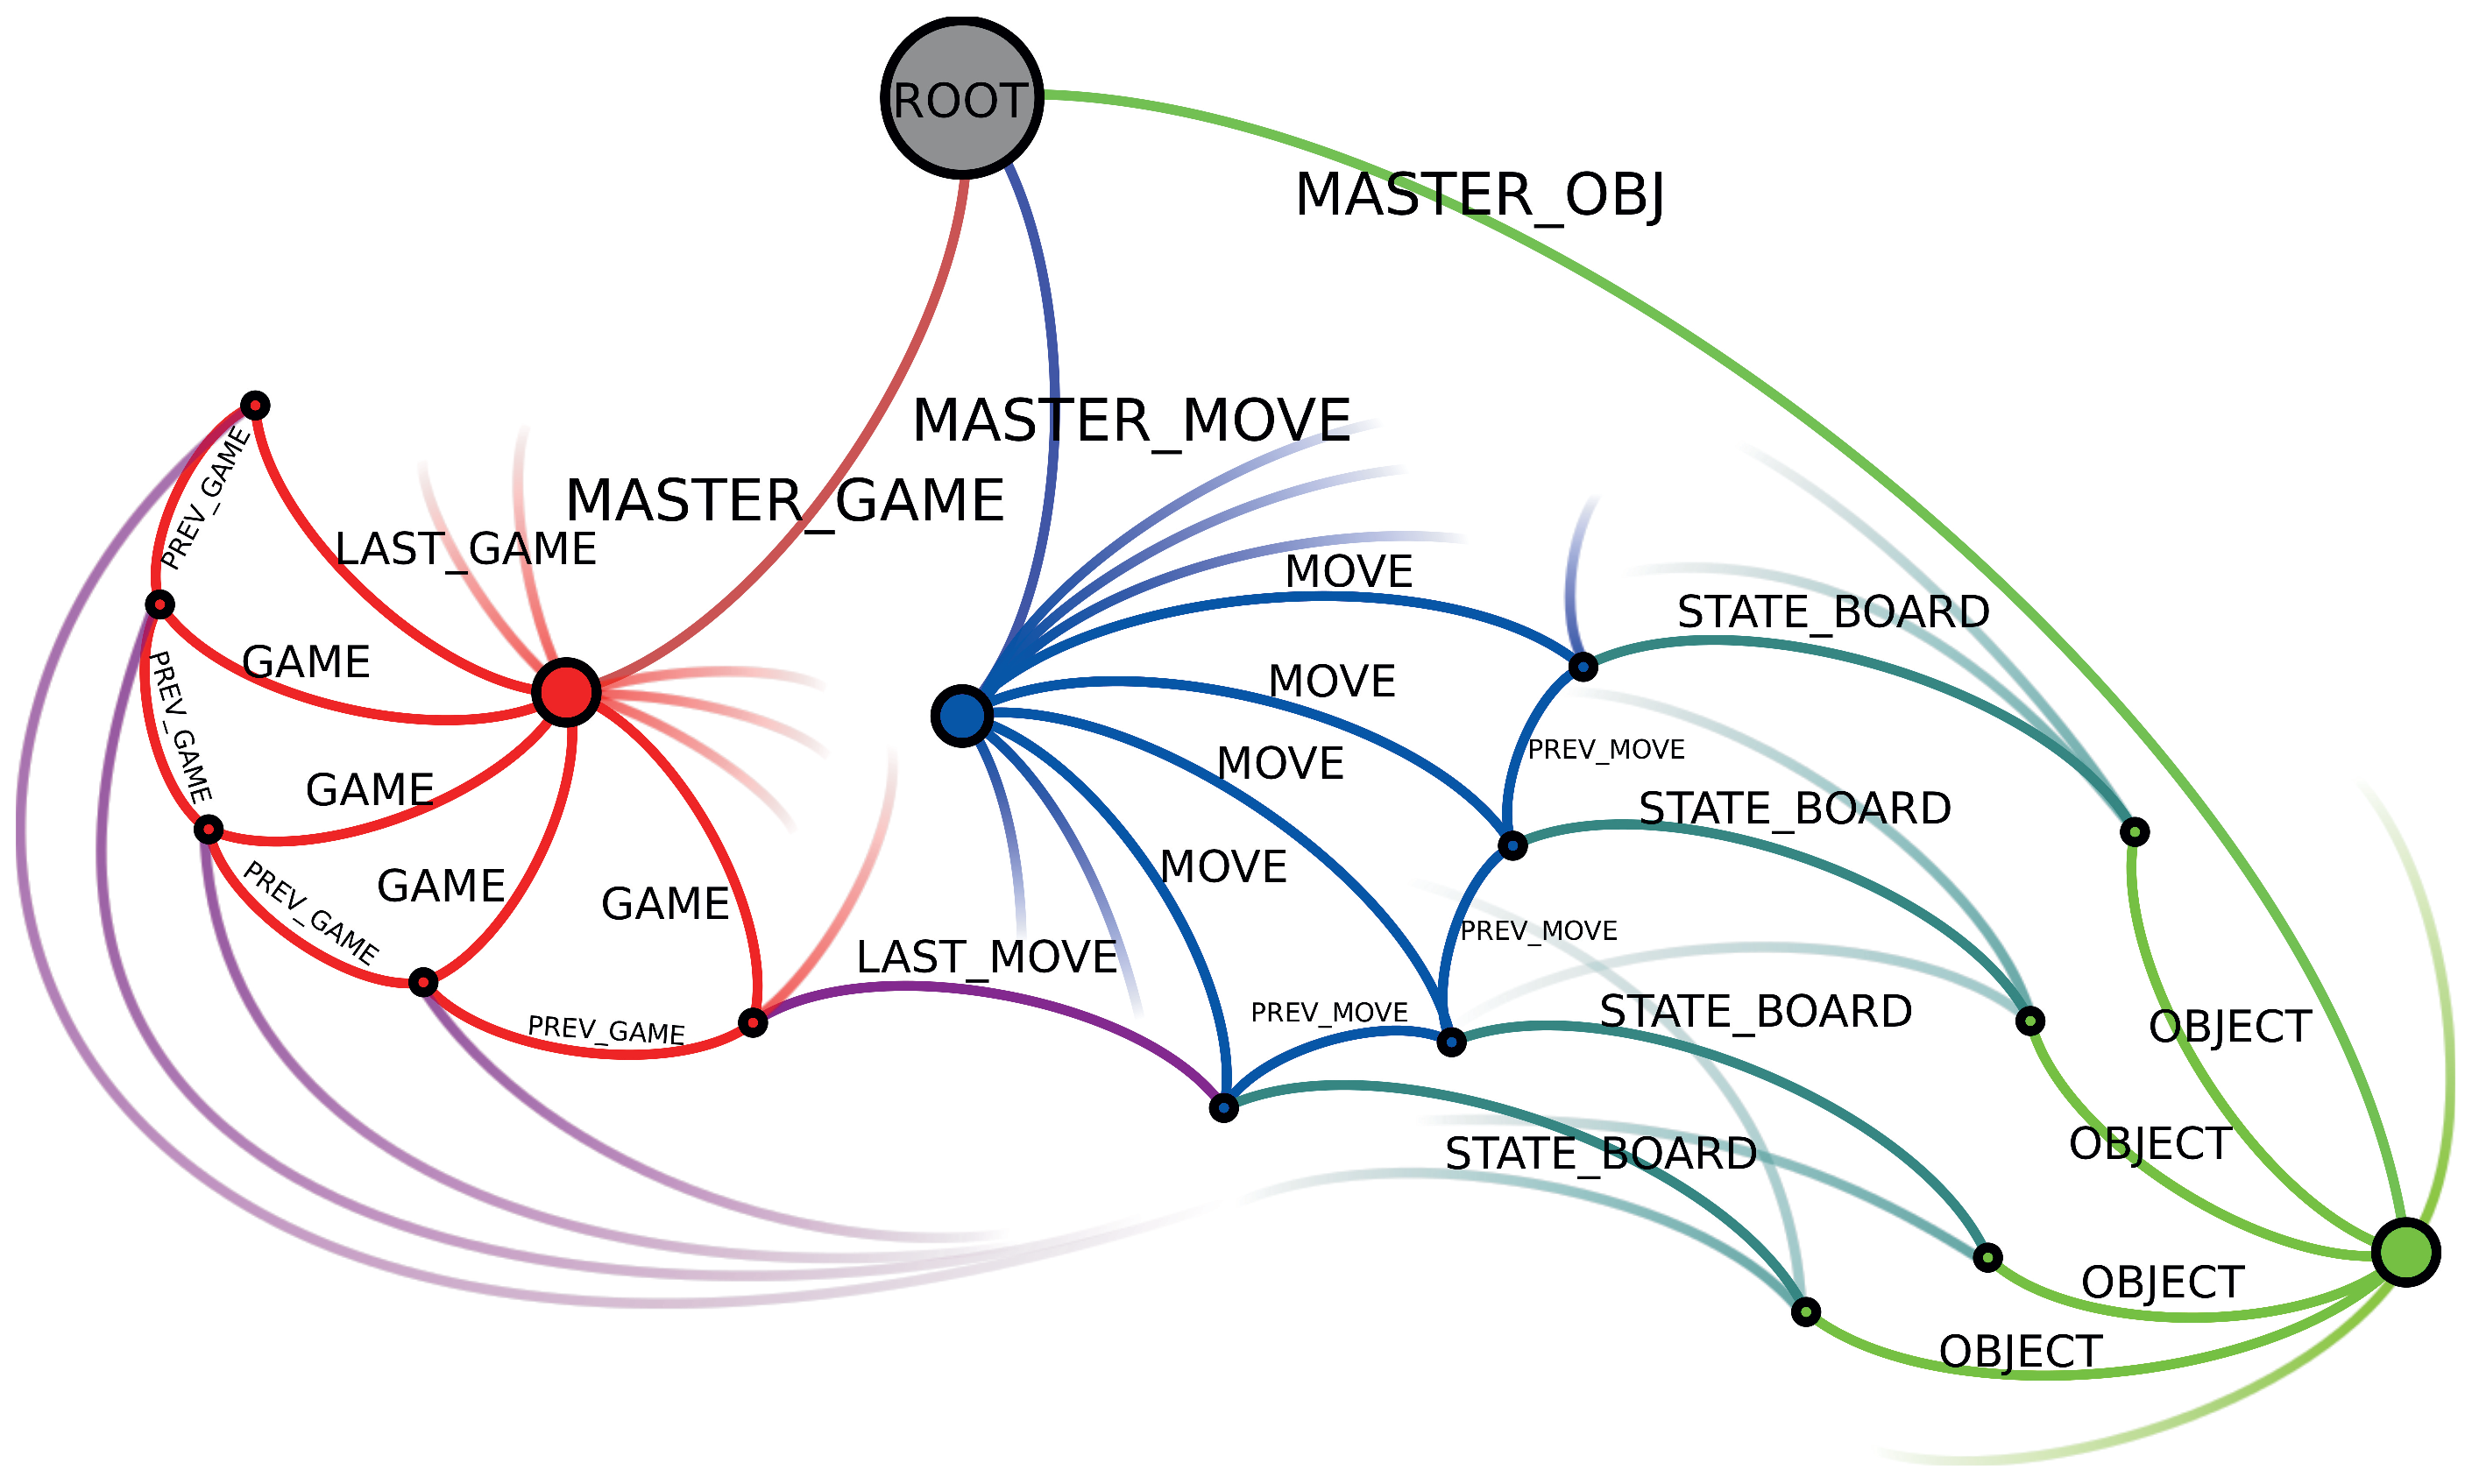
\includegraphics[width=\textwidth]{files/neo4j/episodic_graph}
\caption{Représentation de la mémoire épisodique dans Neo4j.}
\label{episodic_graph}
\end{figure}

\subsubsection{Vision globale de la mémoire}

La figure~\ref{full_graph} présente le stockage de la mémoire épisodique et de la mémoire sémantique dans Neo4j. Les relations de type \texttt{BOARD\_STATE} assure la liaison entre ces deux mémoires.
\begin{figure}[H]
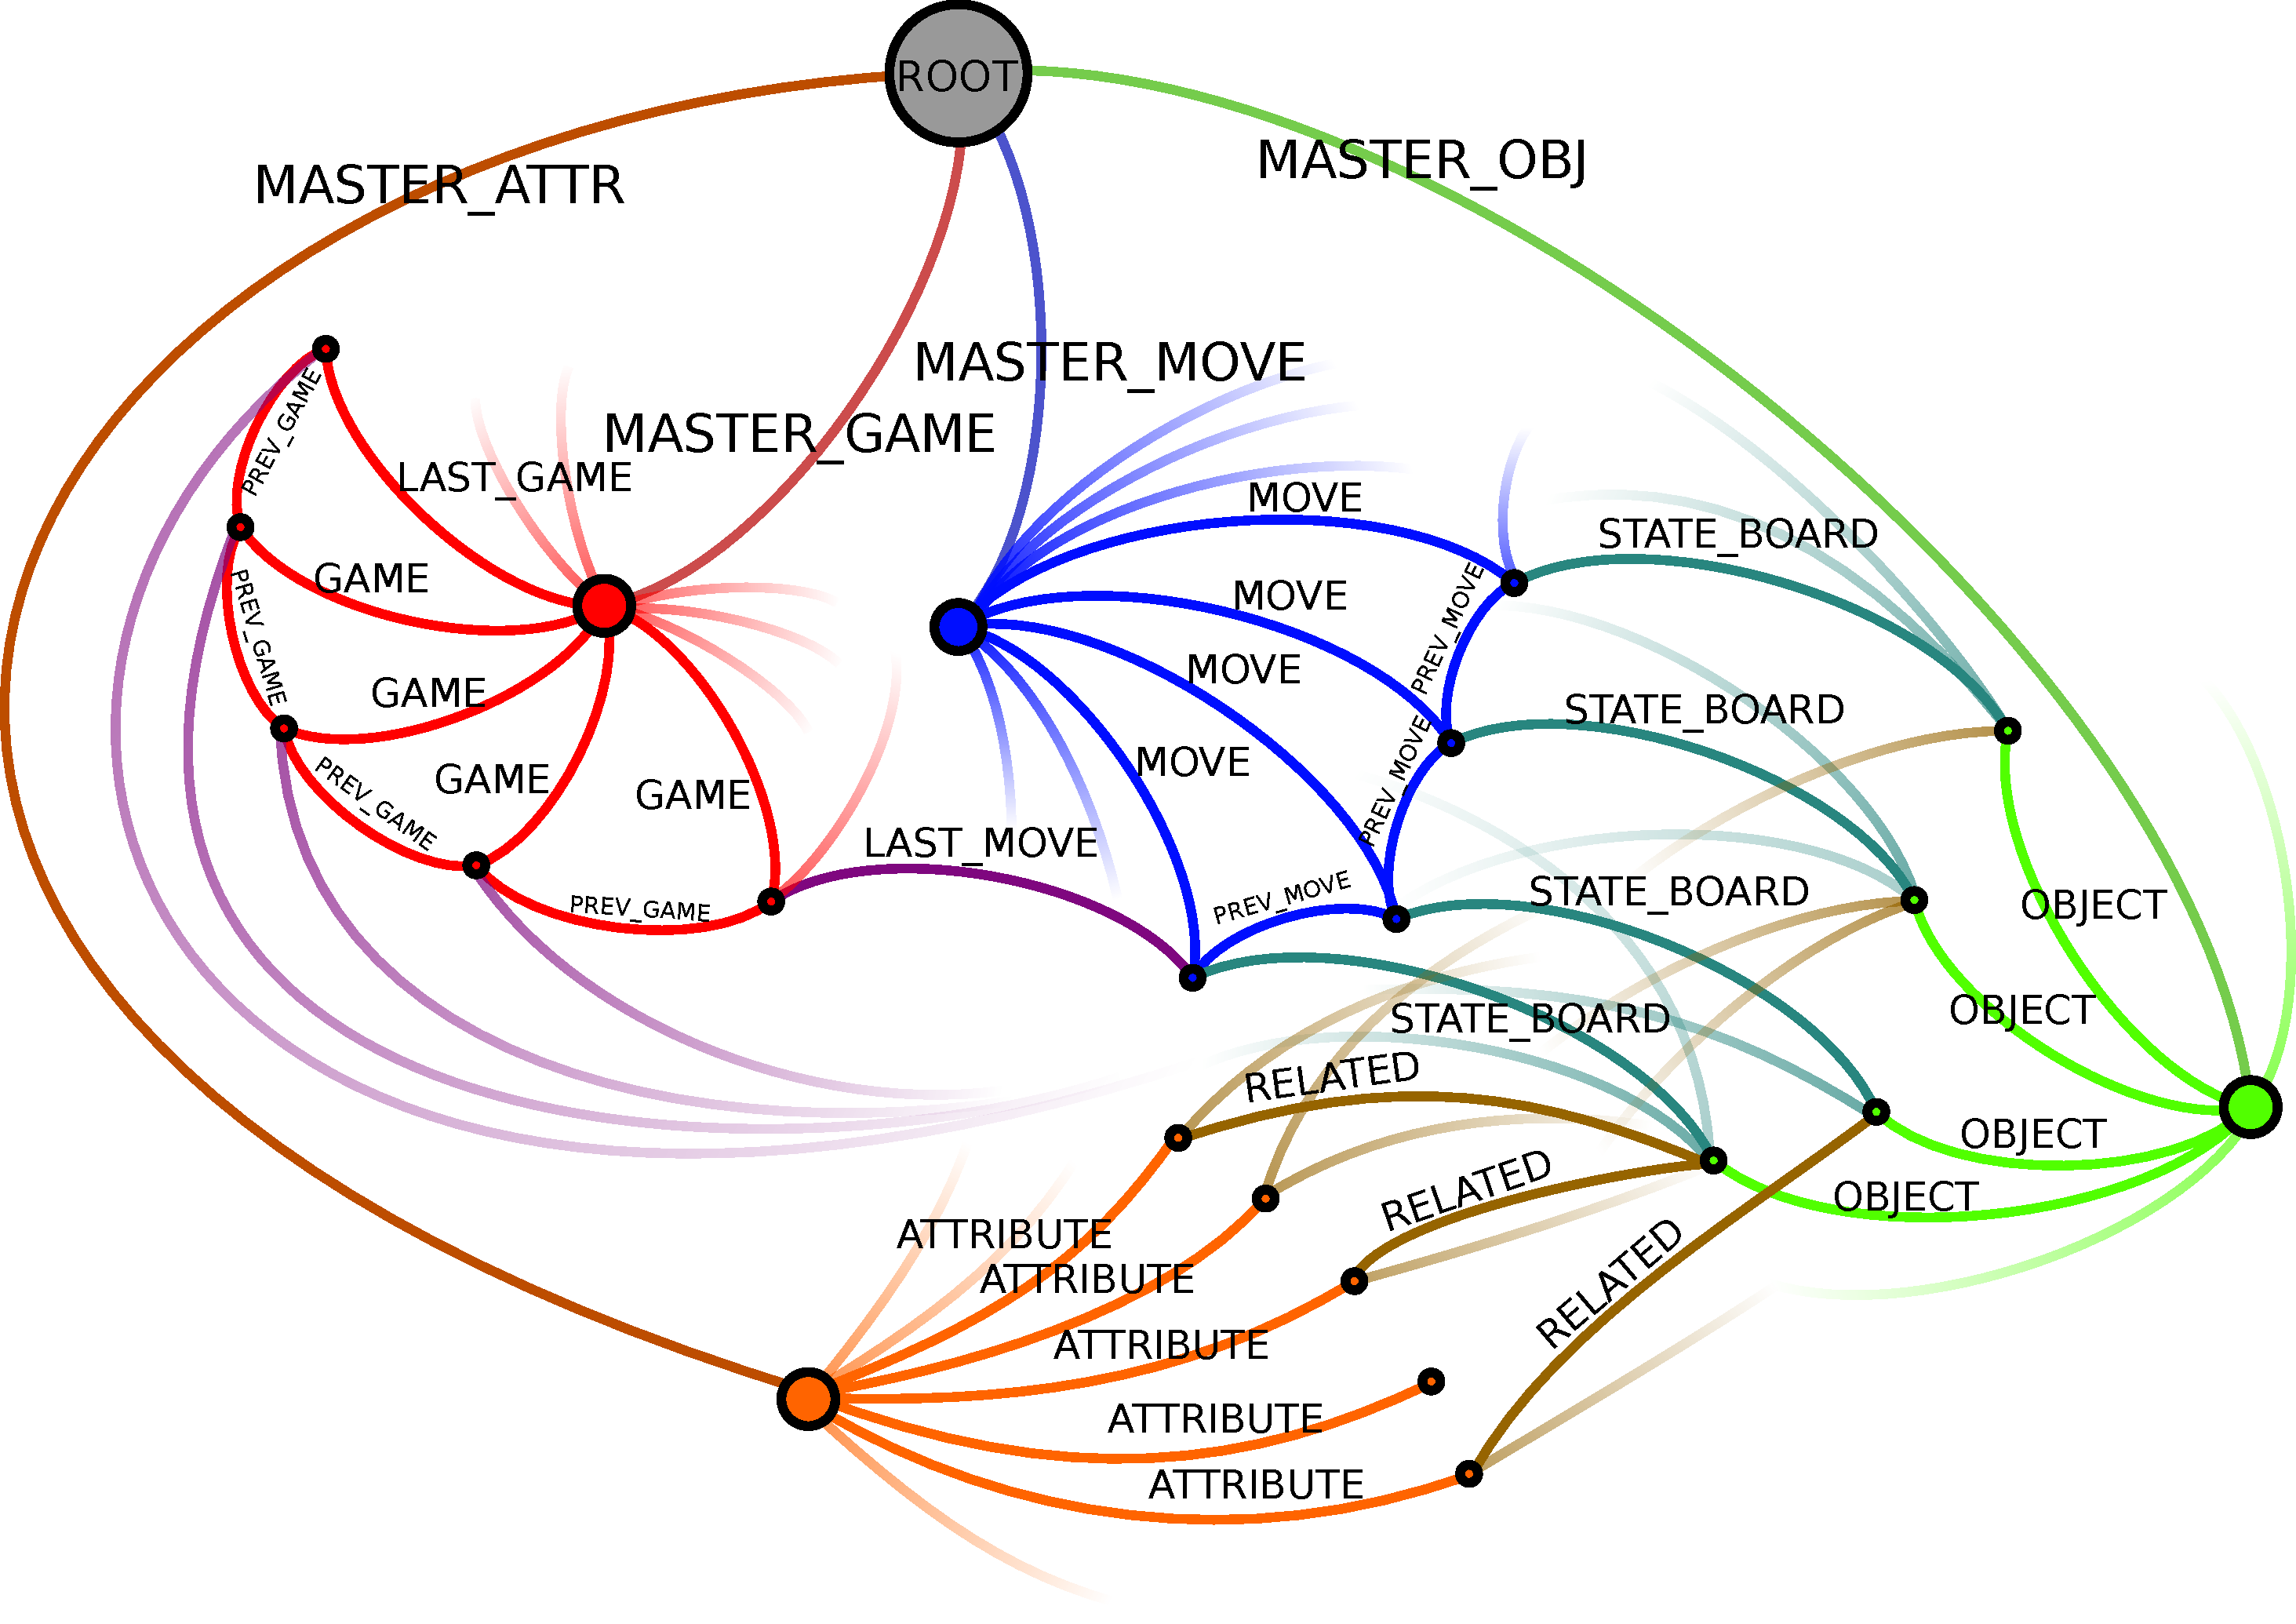
\includegraphics[width=\textwidth]{files/neo4j/full_graph}
\caption{Représentation complète de la mémoire stockée dans Neo4j.}
\label{full_graph}
\end{figure}
Cette première phase d'analyse à consisté en l'étude du modèle de Conscience Artificielle proposé par Guillaume Tisserant. Chaque membre du groupe a commencé par examiner le document. La majorité des décisions prises par rapport aux contraintes relevant du projet dans sa globalité, nous avons choisi de traiter ces questions collectivement. De nombreuses réunions ont donc été organisées entre les membres de l'équipe, au moins deux fois par semaine, et avec nos encadrants, environ une fois par semaine.


\clearemptydoublepage
\begin{frame}{Outils de travail}{Plateforme / Javadoc}

\end{frame}
\clearemptydoublepage
\clearemptydoublepage
\chapter{Résultats \&  discussion}

\section{Résultats}



\section{Discussion}
\subsection{Un treillis en mémoire ?}
Comme nous l'avons vu dans la partie~\ref{conception_memoire_semantique} (page \pageref{conception_memoire_semantique}), la mémoire sémantique entrepose une matrice de booléens associant des formes remarquables à des plateaux. Ces associations correspondent typiquement à la définition d'un contexte, permettant la construction d'un treillis de concepts.

\subsubsection{Analyse de concepts formels}
FCA\footnote{Formal Concept Analysis (en Français \og Analyse de Concepts Formels \fg{}).} est l'étude de concepts définis de manière formelle, via un contexte. Cette section ne présente pas en détail FCA. Pour plus d'informations sur cette méthode d'analyse et les treillis de Galois nous vous recommandons la lecture des cours de Marianne Huchard et de Michel Liquière\footnote{Cours de Marianne Huchard, Professeur en informatique à l'université Montpellier 2 (Faculté des Sciences) et Directrice adjointe du LIRMM (Laboratoire d'Informatique, de Robotique et de Microélectronique de Montpellier) et de Michel Liquière, Maitre de Conférences dans la même université, disponibles à l'adresse suivante : \texttt{http://www.lirmm.fr/\textasciitilde huchard/Huchard/teaching.html}}.

\paragraph{Le contexte} Il s'agit d'un triplet $(G,M,I)$ avec $G$ et $M$ des ensembles et $I\subseteq G \times M$ des relations de $G$ dans $M$. Les éléments contenus dans $G$ sont appelés \emph{objets} et ceux de $M$ \emph{attributs}. $I$ est une relation entre une object de $G$ et un attribut de $M$, et qui se dit \og l'objet $g$ possède l'attribut $m$ \fg{}. (Source : Wikpiedia\footnote{L'article \og Analyse de concepts formels \fg{} de Wikipedia en Français à considérablement aidé à la rédaction de cette partie. Contenu sous licence CC-BY-SA.})

En application à \emph{COGITO} nous aurions :

\begin{tabular}{r c l}
$G$ & $ = $ & ensemble des plateaux (objets),\\
$M$ & $ = $ & ensemble des formes remarquables (attributs),\\
$I$ & $ = $ & ensemble des relations plateaux / formes remarquables\\
& & définies dans la matrice actuelle.\\
\end{tabular}

Construire des concepts à partir du contexte formel permettrait de raisonner à un niveau d'abstraction supplémentaire. Actuellement \emph{COGITO} travail sur des formes remarquables, après la construction d'un treillis de Galois, il pourrait raisonner sur des ensembles de formes remarquables.


\clearemptydoublepage

\pagebreak
 
\addcontentsline{toc}{chapter}{Glossaire}
\printglossary
\pagebreak
 
\addcontentsline{toc}{chapter}{Table des figures}
\listoffigures

\end{document}
